\documentclass[12pt,]{article}
%\usepackage{lmodern}  Melissa removed to deal with font rendering issue
\usepackage{amssymb,amsmath}
\usepackage{ifxetex,ifluatex}
\usepackage{fixltx2e} % provides \textsubscript

%Melissa removed the following section to deal with font rendering issue
%\ifnum 0\ifxetex 1\fi\ifluatex 1\fi=0 % if pdftex
%  \usepackage[T1]{fontenc}
%  \usepackage[utf8]{inputenc}
%%\else % if luatex or xelatex
%  \ifxetex
%    \usepackage{mathspec}
%  \else
%    \usepackage{fontspec}
%  \fi
%  \defaultfontfeatures{Ligatures=TeX,Scale=MatchLowercase}
%  \newcommand{\euro}{€}
%%%%%%\fi

% use upquote if available, for straight quotes in verbatim environments
\IfFileExists{upquote.sty}{\usepackage{upquote}}{}
% use microtype if available
\IfFileExists{microtype.sty}{%
\usepackage{microtype}
\UseMicrotypeSet[protrusion]{basicmath} % disable protrusion for tt fonts
}{}
\usepackage[margin=1in]{geometry}
\usepackage{hyperref}
\PassOptionsToPackage{usenames,dvipsnames}{color} % color is loaded by hyperref
\hypersetup{unicode=true,
            pdftitle={Status of Big Skate (Beringraja binoculata) Off the U.S. Pacific Coast in 2019},
            pdfborder={0 0 0},
            breaklinks=true}
\urlstyle{same}  % don't use monospace font for urls
\usepackage{graphicx,grffile}
\makeatletter
\def\maxwidth{\ifdim\Gin@nat@width>\linewidth\linewidth\else\Gin@nat@width\fi}
\def\maxheight{\ifdim\Gin@nat@height>\textheight\textheight\else\Gin@nat@height\fi}
\makeatother
% Scale images if necessary, so that they will not overflow the page
% margins by default, and it is still possible to overwrite the defaults
% using explicit options in \includegraphics[width, height, ...]{}
\setkeys{Gin}{width=\maxwidth,height=\maxheight,keepaspectratio}
\setlength{\parindent}{0pt}
\setlength{\parskip}{6pt plus 2pt minus 1pt}
\setlength{\emergencystretch}{3em}  % prevent overfull lines
\providecommand{\tightlist}{%
  \setlength{\itemsep}{0pt}\setlength{\parskip}{0pt}}
\setcounter{secnumdepth}{5}

%%% Use protect on footnotes to avoid problems with footnotes in titles
\let\rmarkdownfootnote\footnote%
\def\footnote{\protect\rmarkdownfootnote}

%%% Change title format to be more compact
\usepackage{titling}

% Create subtitle command for use in maketitle
\newcommand{\subtitle}[1]{
  \posttitle{
    \begin{center}\large#1\end{center}
    }
}

\setlength{\droptitle}{-2em}
  \title{Status of Big Skate (\emph{Beringraja binoculata}) Off the U.S. Pacific
Coast in 2019}
  \pretitle{\vspace{\droptitle}\centering\huge}
  \posttitle{\par}
  \author{}
  \preauthor{}\postauthor{}
  \date{}
  \predate{}\postdate{}


% This file contains all of the LaTeX packages you may need to compile the document
% Documentation for each package can be found onlines
\usepackage{tabularx}                                             % table environment providing flexibility
\usepackage{caption}                                              % for creating captions  
\usepackage{longtable}                                            % allows tables to span multiple pages
\usepackage{rotating}                                             % allows for sideways tables
\usepackage{float}                                                % floating environments; may not need in rmarkdown
\usepackage{placeins}                                             % keeps floats from moving
\usepackage{indentfirst}                                          % indents first paragraph of a section
\usepackage{mdwtab}                                               % continued float multi-page figure
\usepackage{enumerate}                                            % create lists
\usepackage{hyperref}                                             % highlight cross references
\hypersetup{colorlinks=true, urlcolor=blue, linktoc=page, linkcolor=blue, citecolor=blue} %define referencing colors
%\usepackage{makebox}                                             % make boxes around text
\usepackage[usenames,dvipsnames]{xcolor}                          % color name options
%\usepackage[space]{grffile}                                      % spaces in file name path
\usepackage{soul}                                                 % highlight text
\usepackage{enumitem}                                             % numbered lists
\usepackage{lineno}                                               % Line numbers; comment out for final
\usepackage{upquote}                                              % produce grave accent in latex
\usepackage{verbatim}                                             % produces verbatim results
\usepackage{fancyvrb}                                             % verbatim in a box
%\usepackage{draftwatermark}                                      % places Draft watermark in background; comment out for final
\usepackage{textcomp}                                             % fixes error with packages interfering
\usepackage{pdflscape}                                               % rotate pages - to allow for landscape longtables
%\pdfinterwordspaceon                                             % fix loss of inter word spacing
\usepackage{cmap}                                                 % fix mapping characters to unicode
\RequirePackage[linewidth = 1]{pdfcomment}                        % pdf comments
\RequirePackage[l2tabu, orthodox]{nag}                            % checks packages related to the accessibility?
%\usepackage[inline]{showlabels}                                   % show table and figure labels; comment out for final
%\RequirePackage[tagged]{accessibilityMeta}
\usepackage{booktabs}                                             % For multi-header tables
\usepackage{geometry}                                             % For landscape display
\usepackage{graphicx}

% \linenumbers                                                      % specify use of line numbers


\definecolor{light-gray}{gray}{.85}                               % define light-gray as a color
%\usepackage[tagged]{accessibility-meta}

 
%\showlabels[\color{mred}]{label}

% Redefines (sub)paragraphs to behave more like sections
\ifx\paragraph\undefined\else
\let\oldparagraph\paragraph
\renewcommand{\paragraph}[1]{\oldparagraph{#1}\mbox{}}
\fi
\ifx\subparagraph\undefined\else
\let\oldsubparagraph\subparagraph
\renewcommand{\subparagraph}[1]{\oldsubparagraph{#1}\mbox{}}
\fi

\begin{document}
\maketitle


\begin{center}
\thispagestyle{empty}

\vspace{.7cm}

% 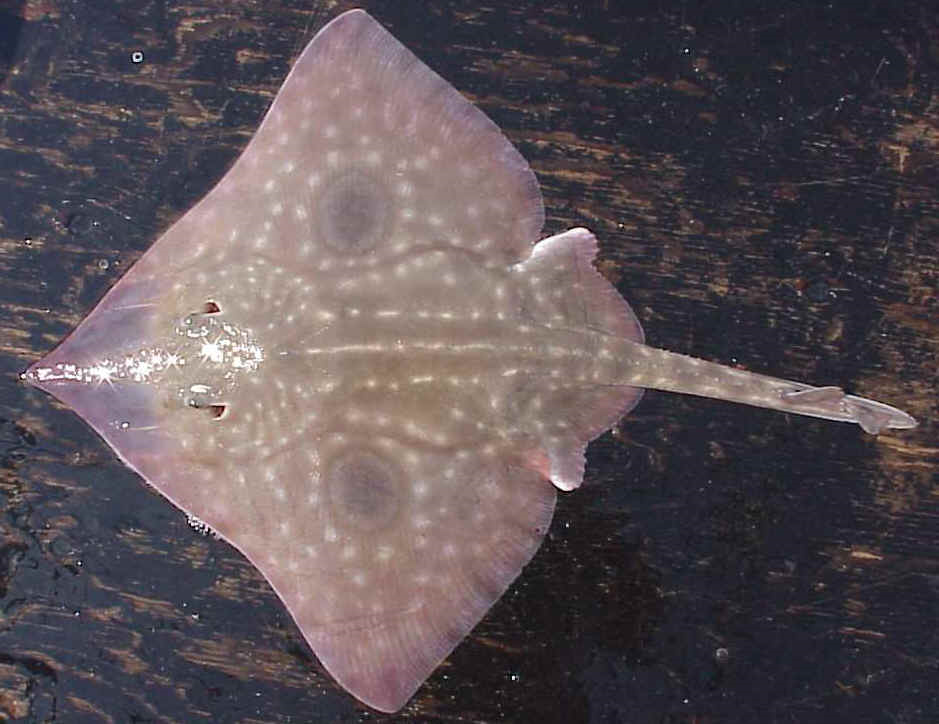
\includegraphics{cover_photo}~\\[1cm]
\pdftooltip{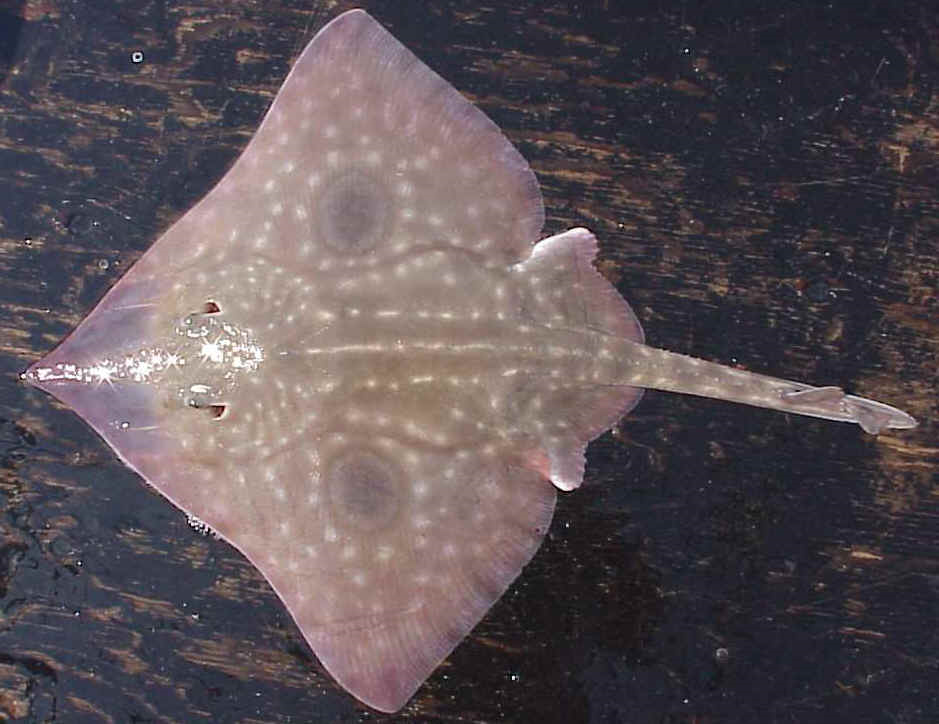
\includegraphics{cover_photo}}{This is a fish.}

\vspace{.5cm}

Ian G. Taylor\textsuperscript{1}\\
Vladlena Gertseva\textsuperscript{1}\\
Andi Stephens\textsuperscript{2}\\
Joseph Bizzarro\textsuperscript{3}\\

\vspace{.7cm}

\small

\textsuperscript{1}Northwest Fisheries Science Center, U.S. Department of Commerce, National Oceanic and Atmospheric Administration, National Marine Fisheries Service, 2725 Montlake Boulevard East, Seattle, Washington 98112\\

\vspace{.3cm}

\textsuperscript{2}Northwest Fisheries Science Center, U.S. Department of Commerce, National Oceanic and Atmospheric Administration, National Marine Fisheries Service, 2032 S.E. OSU Drive Newport, Oregon 97365

\vspace{.3cm}

\textsuperscript{3}Southwest Fisheries Science Center, U.S. Department of Commerce, National Oceanic and Atmospheric Administration, National Marine Fisheries Service, 110 Shaffer Road, Santa Cruz, California 95060\\



\vspace{.5cm}

\vfill
DRAFT SAFE\\
Disclaimer: This information is distributed solely for the purpose of pre-dissemination
peer review under applicable information quality guidelines. It has not been formally
disseminated by NOAA Fisheries. It does not represent and should not be construed to
represent any agency determination or policy. 

\vspace{.3cm}
%Bottom of the page
%{\large \today}


\newpage{\thispagestyle{empty}}

\vspace*{\fill}
\begin{flushleft}
This report may be cited as:

Taylor, I.G., Gertseva, V., Stephens, A. and Bizzarro, J. Status of Big Skate (\emph{Beringraja binoculata}) Off the U.S. West Coast, 2019. Pacific Fishery Management Council, Portland, OR. Available from http://www.pcouncil.org/groundfish/stock-assessments/
\end{flushleft}

\newpage{\thispagestyle{empty}}

% Create this table using the instructions in Acronyms.Rmd


\begin{flushleft}
\large{\textbf{Acronyms used in this Document}}
\end{flushleft}

\vspace{.5cm}

\renewcommand{\arraystretch}{1.2}

\begin{table}[ht]
% \centering
\begin{tabular}{rll}
\hline
 &  ABC & Allowable Biological Catch \\ 
 &  ACL & Annual Catch Limit \\ 
 &  AFSC & Alaska Fisheries Science Center \\ 
 &  CDFW & California Department of Fish and Wildlife \\ 
 &  DFO & Canada's Department of Fisheries and Oceans \\
 &  DW & Disk Width \\
 &  IFQ & Individual Fishing Quota \\
 &  IPHC & International Pacific Halibut Commission \\
 &  ISW & Interspiracular Width \\
 &  NMFS & National Marine Fisheries Service \\
 &  NWFSC & Northwest Fisheries Science Center \\
 &  ODFW & Oregon Department of Fish and Wildlife \\
 &  OFL & Overfishing Limit \\
 &  OY & Optimum Yield \\
 &  PacFIN & Pacific Fisheries Information Network \\
 &  PFMC & Pacific Fishery Management Council \\
 &  SPR & Spawning Potential Ratio \\
 &  SSC & Scientific and Statistical Committee \\
 &  SWFSC & Southwest Fisheries Science Center \\
 &  TL & Total Length \\
 &  VAST & Vector Autoregressive Spatio-Temporal Package \\
 &  WCGBT & West Coast Groundfish Bottom Trawl Survey \\
 &  WCGOP & West Coast Groundfish Observer Program \\
 &  WDFW & Washington Department of Fish and Wildlife \\
   \hline
\end{tabular}
\end{table}

\renewcommand{\arraystretch}{1}

\maketitle

\pagenumbering{roman}
\setcounter{page}{1}
\end{center}

{
\setcounter{tocdepth}{4}
\tableofcontents
}
\setlength{\parskip}{5mm plus1mm minus1mm}
\pagebreak

\pagenumbering{roman}

\renewcommand{\thefigure}{\alph{figure}}
\renewcommand{\thetable}{\alph{table}}

\hypertarget{executive-summary}{%
\section*{Executive Summary}\label{executive-summary}}
\addcontentsline{toc}{section}{Executive Summary}

\hypertarget{stock}{%
\subsection*{Stock}\label{stock}}
\addcontentsline{toc}{subsection}{Stock}

This assessment reports the status of the Big Skate
(\emph{Beringraja binoculata}) resource in U.S. waters off the West
Coast using data through 2018. A map showing the area of the U.S. West
Coast Exclusive Economic Zone covered by this stock assessment is
provided in Figure \ref{fig:assess_region_map}.

\begin{figure}[H]
\begin{centering}
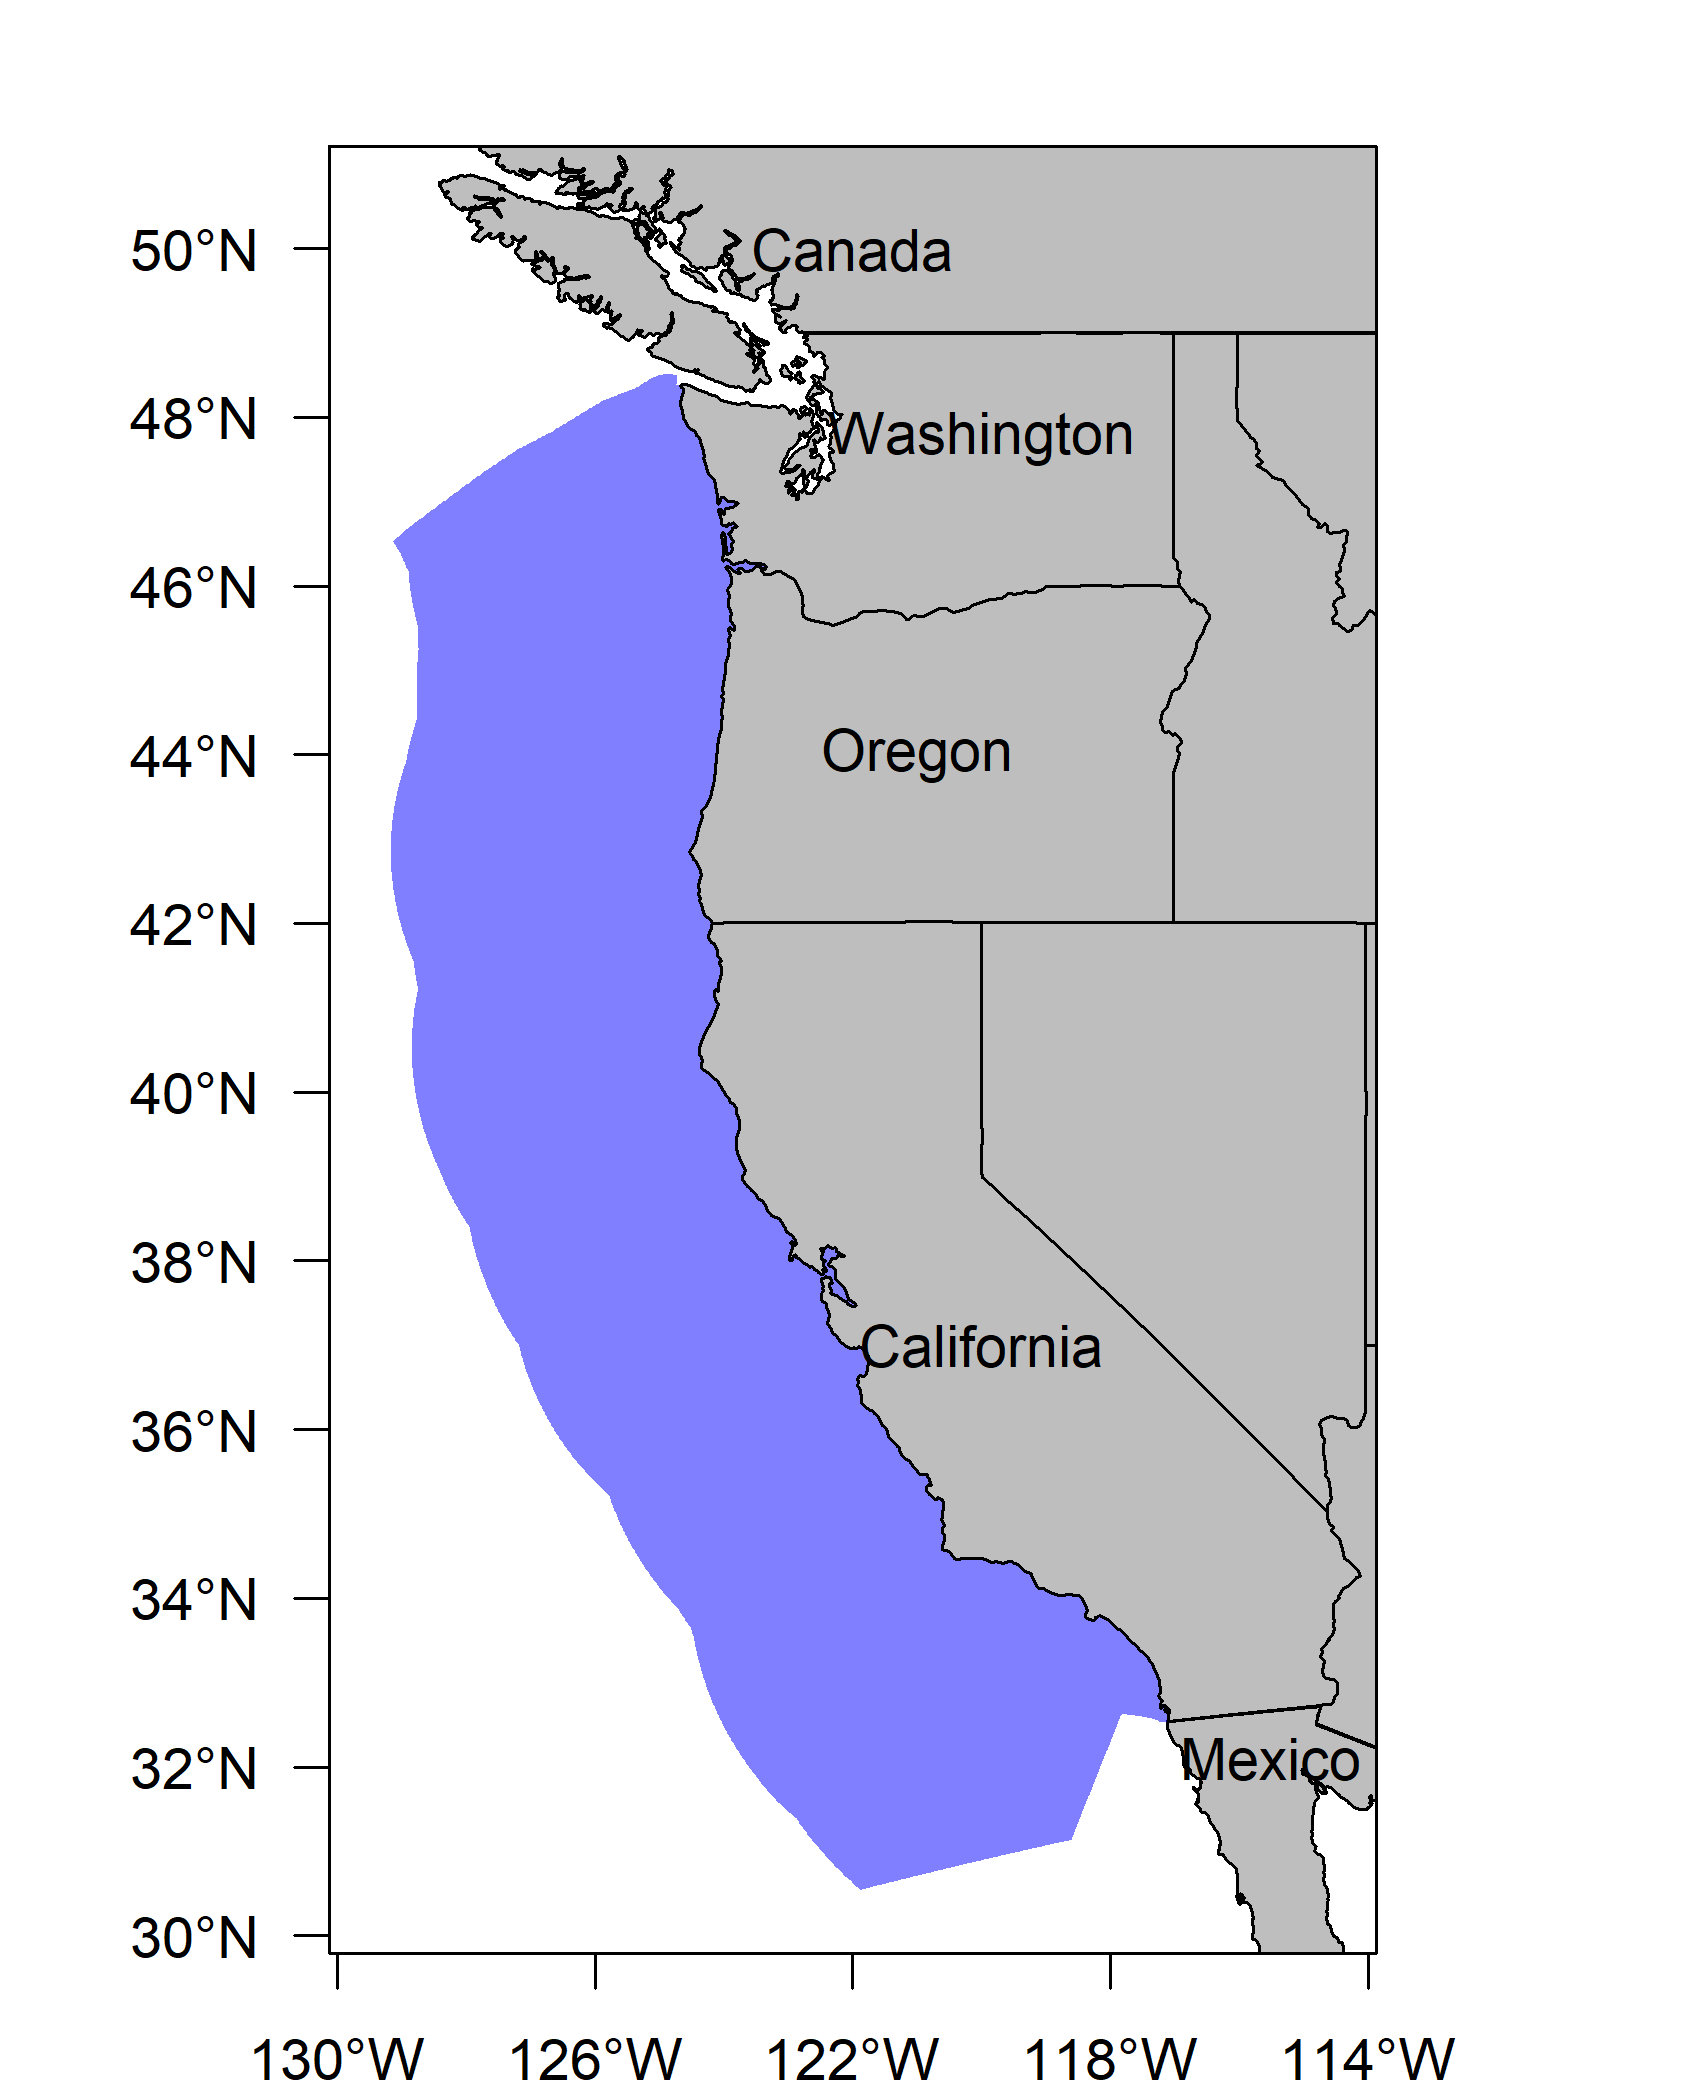
\includegraphics{Figures/assess_region_map.png}
\caption{U.S. West Coast Exclusive Economic zone covering the area in which this stock assessment is focused.}\label{fig:assess_region_map}
\end{centering}
\end{figure}

\hypertarget{catches}{%
\subsection*{Catches}\label{catches}}
\addcontentsline{toc}{subsection}{Catches}

The majority of Big Skate catch was discarded prior to 1995 when markets
for Big Skate and Longnose Skate developed, landings increased, and
discarding decreased. The majority of the discards were unrecorded and
the landings were in the unspecified skates category. The landings from
prior to 1995 were reconstructed separately in each of the three coastal
states for this assessment. In general the methods all relied on
differences in depth distribution of the different skates species
(primarily Big Skate and Longnose Skate). Discards during this period
prior to 1995 were estimated outside the model based on an assumption
that the average discard rate during the period 1950--1994 was equal to
that for Longnose Skate. The current fishery, beginning in 1995, has
less uncertainty in landings, lower discard rates, and more data on
discards. The discards are estimated within the model for this period
using a time-varying retention function. Big Skate have only been landed
in their own species category in the past few years (starting in 2015).

In the current fishery (since 1995), annual total landings of Big Skate
have ranged between 135-528 mt, with landings in 2018 totaling 173 mt.

\vspace{.5cm}

\FloatBarrier

\begin{table}[ht]
\centering
\caption{Recent Big Skate landings (mt)} 
\label{tab:Exec_catch}
\begin{tabular}{>{\centering}p{1in}>{\centering}p{1in}}
  \hline
Year & Landings \\ 
  \hline
2008 & 366.0 \\ 
  2009 & 205.7 \\ 
  2010 & 196.2 \\ 
  2011 & 268.4 \\ 
  2012 & 269.6 \\ 
  2013 & 135.0 \\ 
  2014 & 372.4 \\ 
  2015 & 331.5 \\ 
  2016 & 411.5 \\ 
  2017 & 277.6 \\ 
  2018 & 172.6 \\ 
   \hline
\end{tabular}
\end{table}

\FloatBarrier

\begin{figure}
\centering
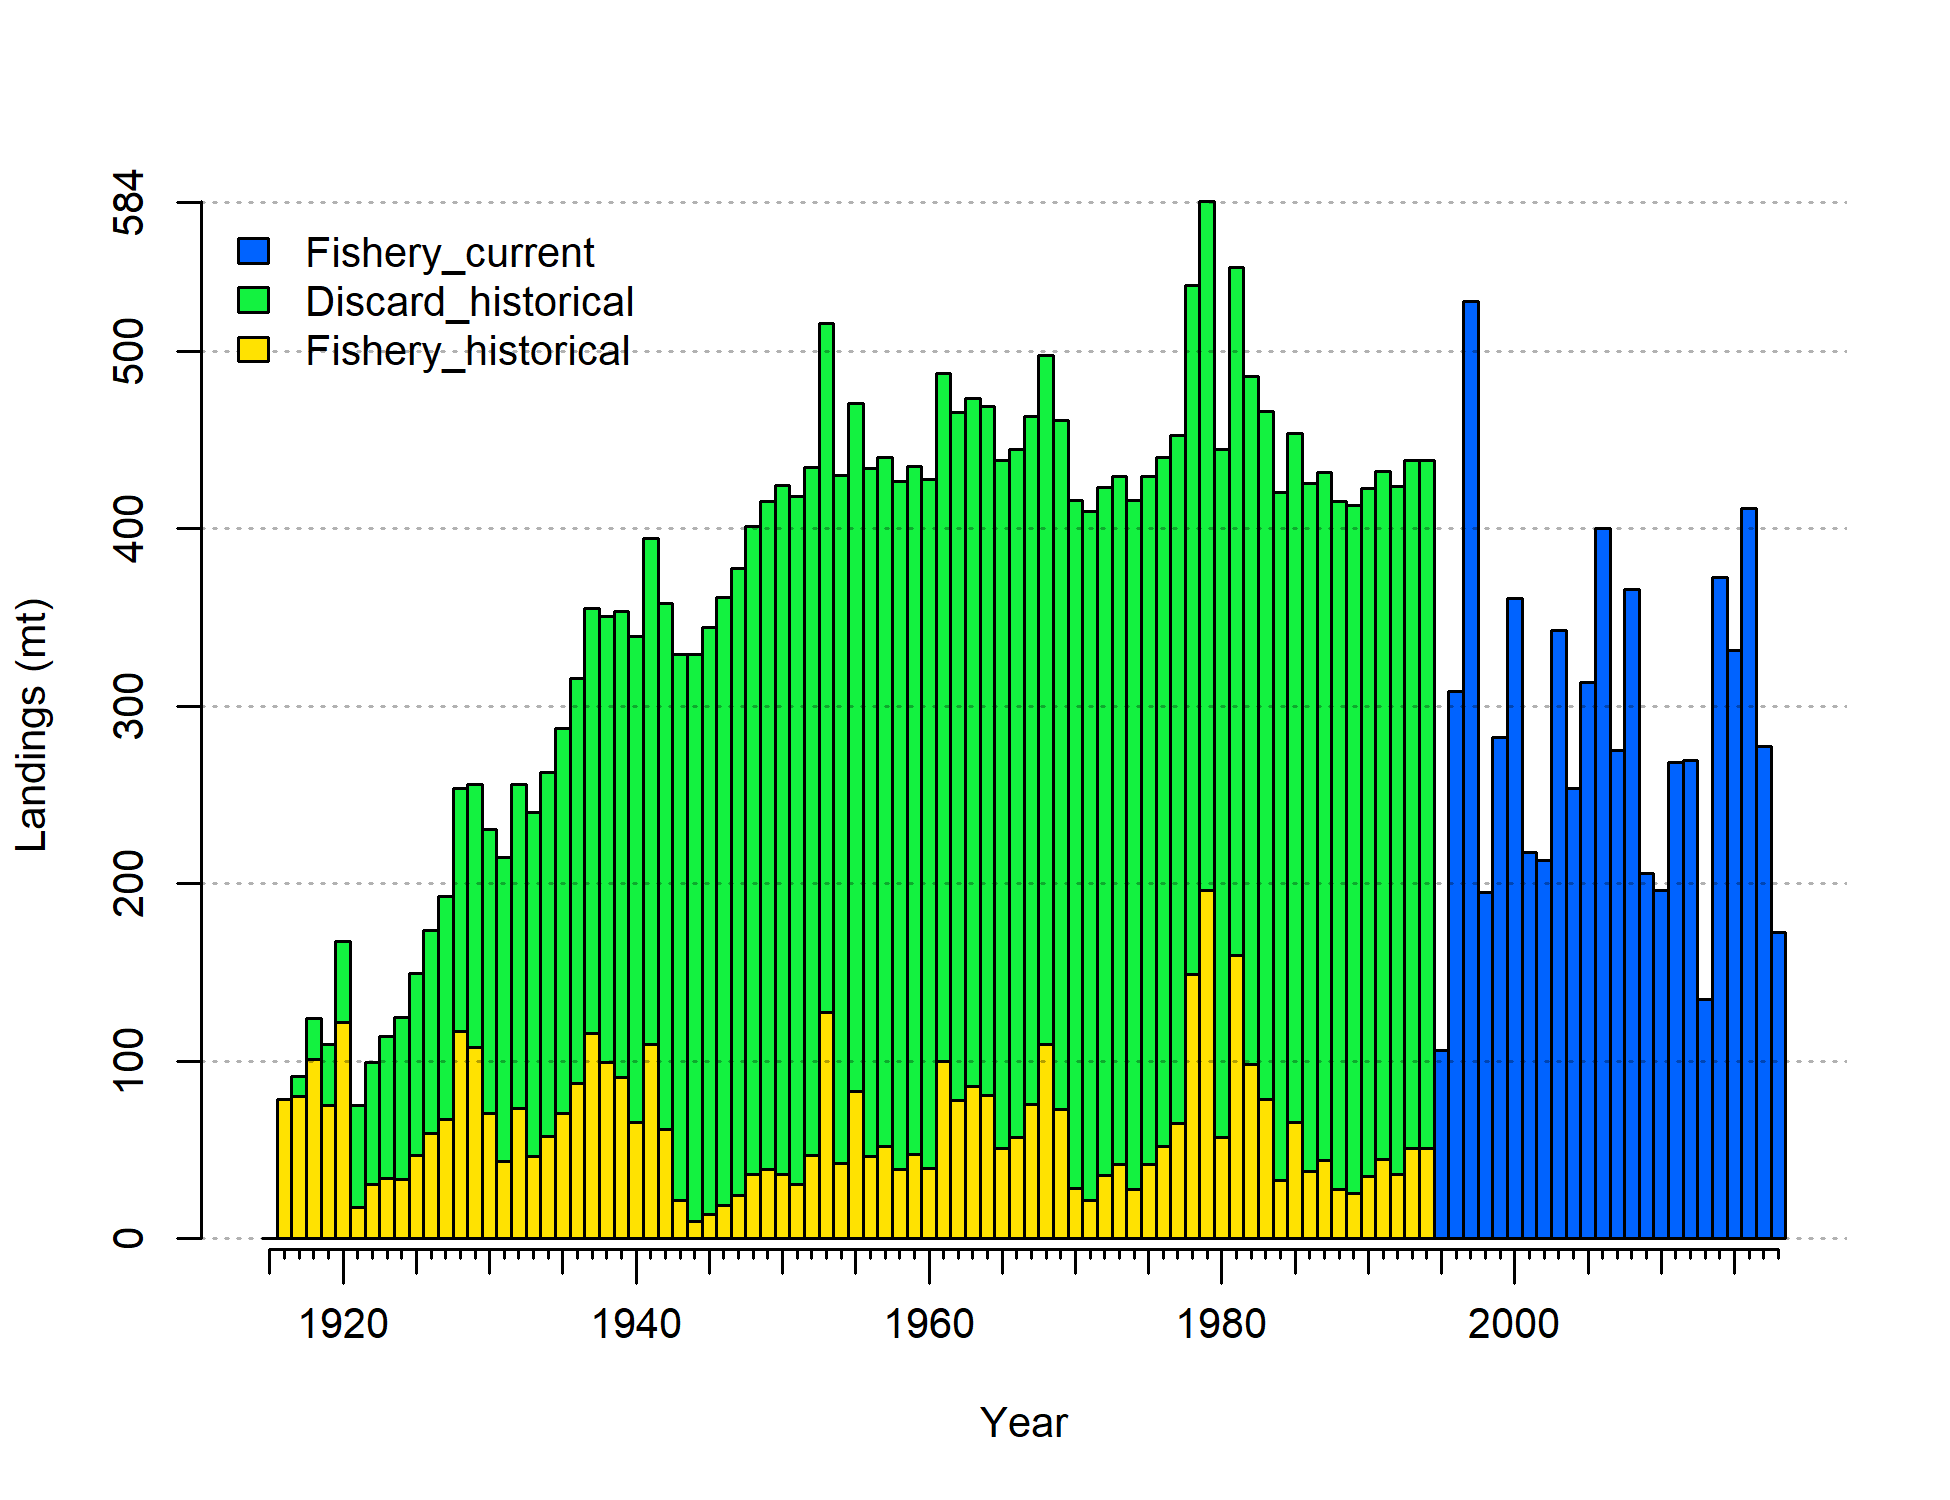
\includegraphics{r4ss/plots_mod1/catch2 landings stacked.png}
\caption{Catch history of Big Skate in the model.
\label{fig:r4ss_catches}}
\end{figure}

\FloatBarrier

\newpage

\hypertarget{data-and-assessment}{%
\subsection*{Data and Assessment}\label{data-and-assessment}}
\addcontentsline{toc}{subsection}{Data and Assessment}

This the first full assessment for Big Skate. It is currently managed
using an OFL which was based on a proxy for \(F_{MSY}\) and the average
survey biomass for the years 2010--2012. This assessment uses the newest
version of Stock Synthesis (3.30.13.02). The model begins in 1916, and
assumes the stock was at an unfished equilibrium that year. The choice
of 1916 is based on the first year of the Califonia catch
reconstruction.

The assessment relies on two bottom trawl survey indices of abundance,
the Triennial Survey from which an index covering the period 1980--2004
was used here and the West Coast Groundfish Bottom Trawl (WCGBT) Survey,
which began in 2003 and for which data is available through 2018. The
triennial survey shows an increasing trend over the 25 year period it
covers, which the model is not able to fit as this includes the period
when trawl fishing in this area was at its most intense and the stock
would is expected to have been declining. The WCGBT Survey also shows an
increasing trend, with the 5 most recent observations (2014--2018) all
falling in the top 6 ever observed (2004 was the 5th highest
observation). The model estimates an increasing trend during this period
but the slope is more gradual than the trend in the survey observations.
The misfit to these survey indices could be due to some combination of
incorrect estimation of the catch history, variability in recruitment
which is not modeled here, or biological or ecological changes which are
not modeled.

Length composition data from the fishery is available starting in 1995
but is sparse until the most recent 10 years. Most of the ages are also
from 2008 onward. This limits the ability of the model to estimate any
changes in composition of the population during the majority of the
history of the fishery. Estimates of discard rates and mean body weight
of discards are available for the years 2002 onward and discard length
compositions are available starting in 2010.

The age and length data provide evidence for growth patterns and
sex-specific differences in selectivity that are unusual among
groundfish stocks that have been assessed within the U.S. West Coast and
are not found in Longnose Skate, where the data show little difference
between the sexes. Growth appears to be almost linear and similar
between females and males up to about age 7 or over 100 cm at which
point male growth appears to stabilize while females continue to grow.
However, in spite of the similar growth pattern for ages prior to 7,
males are observed more frequently in the length bins associated with
these ages, with the 70--100 cm length bins showing more than 60\% males
in many years. Sex-specific differences in selectivity were included in
the model in order to better match patterns in the sex ratios in the
length composition data and a new ``growth cessation model'' was used to
model growth as it provided much better fits than the von Bertalanffy
growth function. The length and age data do not cover enough years or
show enough evidence of distinct cohorts to reliably estimate deviations
in recruitment around the stock-recruit curve, so recruitment in the
final model is based directly on the Beverton-Holt stock-recruit curve.
Steepness of this stock-recruit curve was not well-informed by the model
so was fixed at the value used in a previous Longnose Skate stock
assessment (Gertseva, V and Schirippa, MJ
\protect\hyperlink{ref-Gertseva2007}{2007}).

The final model has 44 estimated parameters, most of which are related
to selectivity (including sex-specific differences), time-varying
retention, and growth (including sex-specific differences). The
remaining 7 parameters include natural mortality, equilibrium
recruitment, an extra survey uncertainty parameter for each of the two
surveys, and three catchability parameters, where the Triennial Survey
is assumed to have a change in catchability starting in 1995 due to
changes in survey design.

The scale of the population is not reliably informed by the data due to
the combination of surveys that show trends which can't be matched by
the structure of the model, and length and age data which inform growth
and selectivity but provide relatively little information about changes
in stock structure over time. Therefore, a prior on catchability of the
WCGBT Survey (centered at 0.83) was applied in order to provide more
stable results.

Although the assessment model requires numerous simplifying assumptions,
it represents an improvement over the simplistic status-quo method of
setting management limits, which relies on average survey biomass and an
assumption about \(F_{MSY}\). The use of an age-structured model with
estimated growth, selectivity, and natural mortality likely provides a
better estimate of past dynamics and the impacts of fishing in the
future.

\hypertarget{stock-biomass}{%
\subsection*{Stock Biomass}\label{stock-biomass}}
\addcontentsline{toc}{subsection}{Stock Biomass}

The 2018 estimated spawning biomass relative to unfished equilibrium
spawning biomass is above the target of 40\% of unfished spawning
biomass at 79.2\% (95\% asymptotic interval: \(\pm\) 65.5\%-92.9\%)
(Figure \ref{fig:Spawnbio_all} and Table
\ref{tab:SpawningDeplete_mod1}). Approximate confidence intervals based
on the asymptotic variance estimates show that the uncertainty in the
estimated spawning biomass is high, although even the lower range of the
95\% interval for \%unfished is above the 40\% reference point, and all
sensitivity analyses explored also show the stock to be at a relatively
high level.

\vspace{.5cm}

\FloatBarrier

\begin{table}[ht]
\centering
\caption{Recent trend in beginning of the 
                                      year spawning output and %unfished
                                      (spawning biomass relative to unfished
                                      equilibrum spawning biomass)} 
\label{tab:SpawningDeplete_mod1}
\begin{tabular}{l>{\centering}p{1.3in}>{\centering}p{1.2in}>{\centering}p{1in}>{\centering}p{1.2in}}
  \hline
Year & Spawning Output (mt) & \~{} 95\% confidence interval & Estimated \%unfished & \~{} 95\% confidence interval \\ 
  \hline
2010 & 1938.7 & (507.5-3369.9) & 0.768 & (0.616-0.92) \\ 
  2011 & 1952.3 & (519.8-3384.9) & 0.773 & (0.624-0.922) \\ 
  2012 & 1960.1 & (527.3-3393) & 0.776 & (0.628-0.924) \\ 
  2013 & 1969.0 & (535.8-3402.1) & 0.780 & (0.634-0.926) \\ 
  2014 & 1991.1 & (556-3426.2) & 0.789 & (0.648-0.93) \\ 
  2015 & 1990.4 & (556.3-3424.5) & 0.788 & (0.647-0.929) \\ 
  2016 & 1992.8 & (559.1-3426.6) & 0.789 & (0.649-0.929) \\ 
  2017 & 1984.9 & (552.5-3417.3) & 0.786 & (0.645-0.927) \\ 
  2018 & 1987.9 & (555.4-3420.4) & 0.787 & (0.647-0.927) \\ 
  2019 & 1999.3 & (565.7-3433) & 0.792 & (0.655-0.929) \\ 
   \hline
\end{tabular}
\end{table}

\FloatBarrier

\begin{figure}
\centering
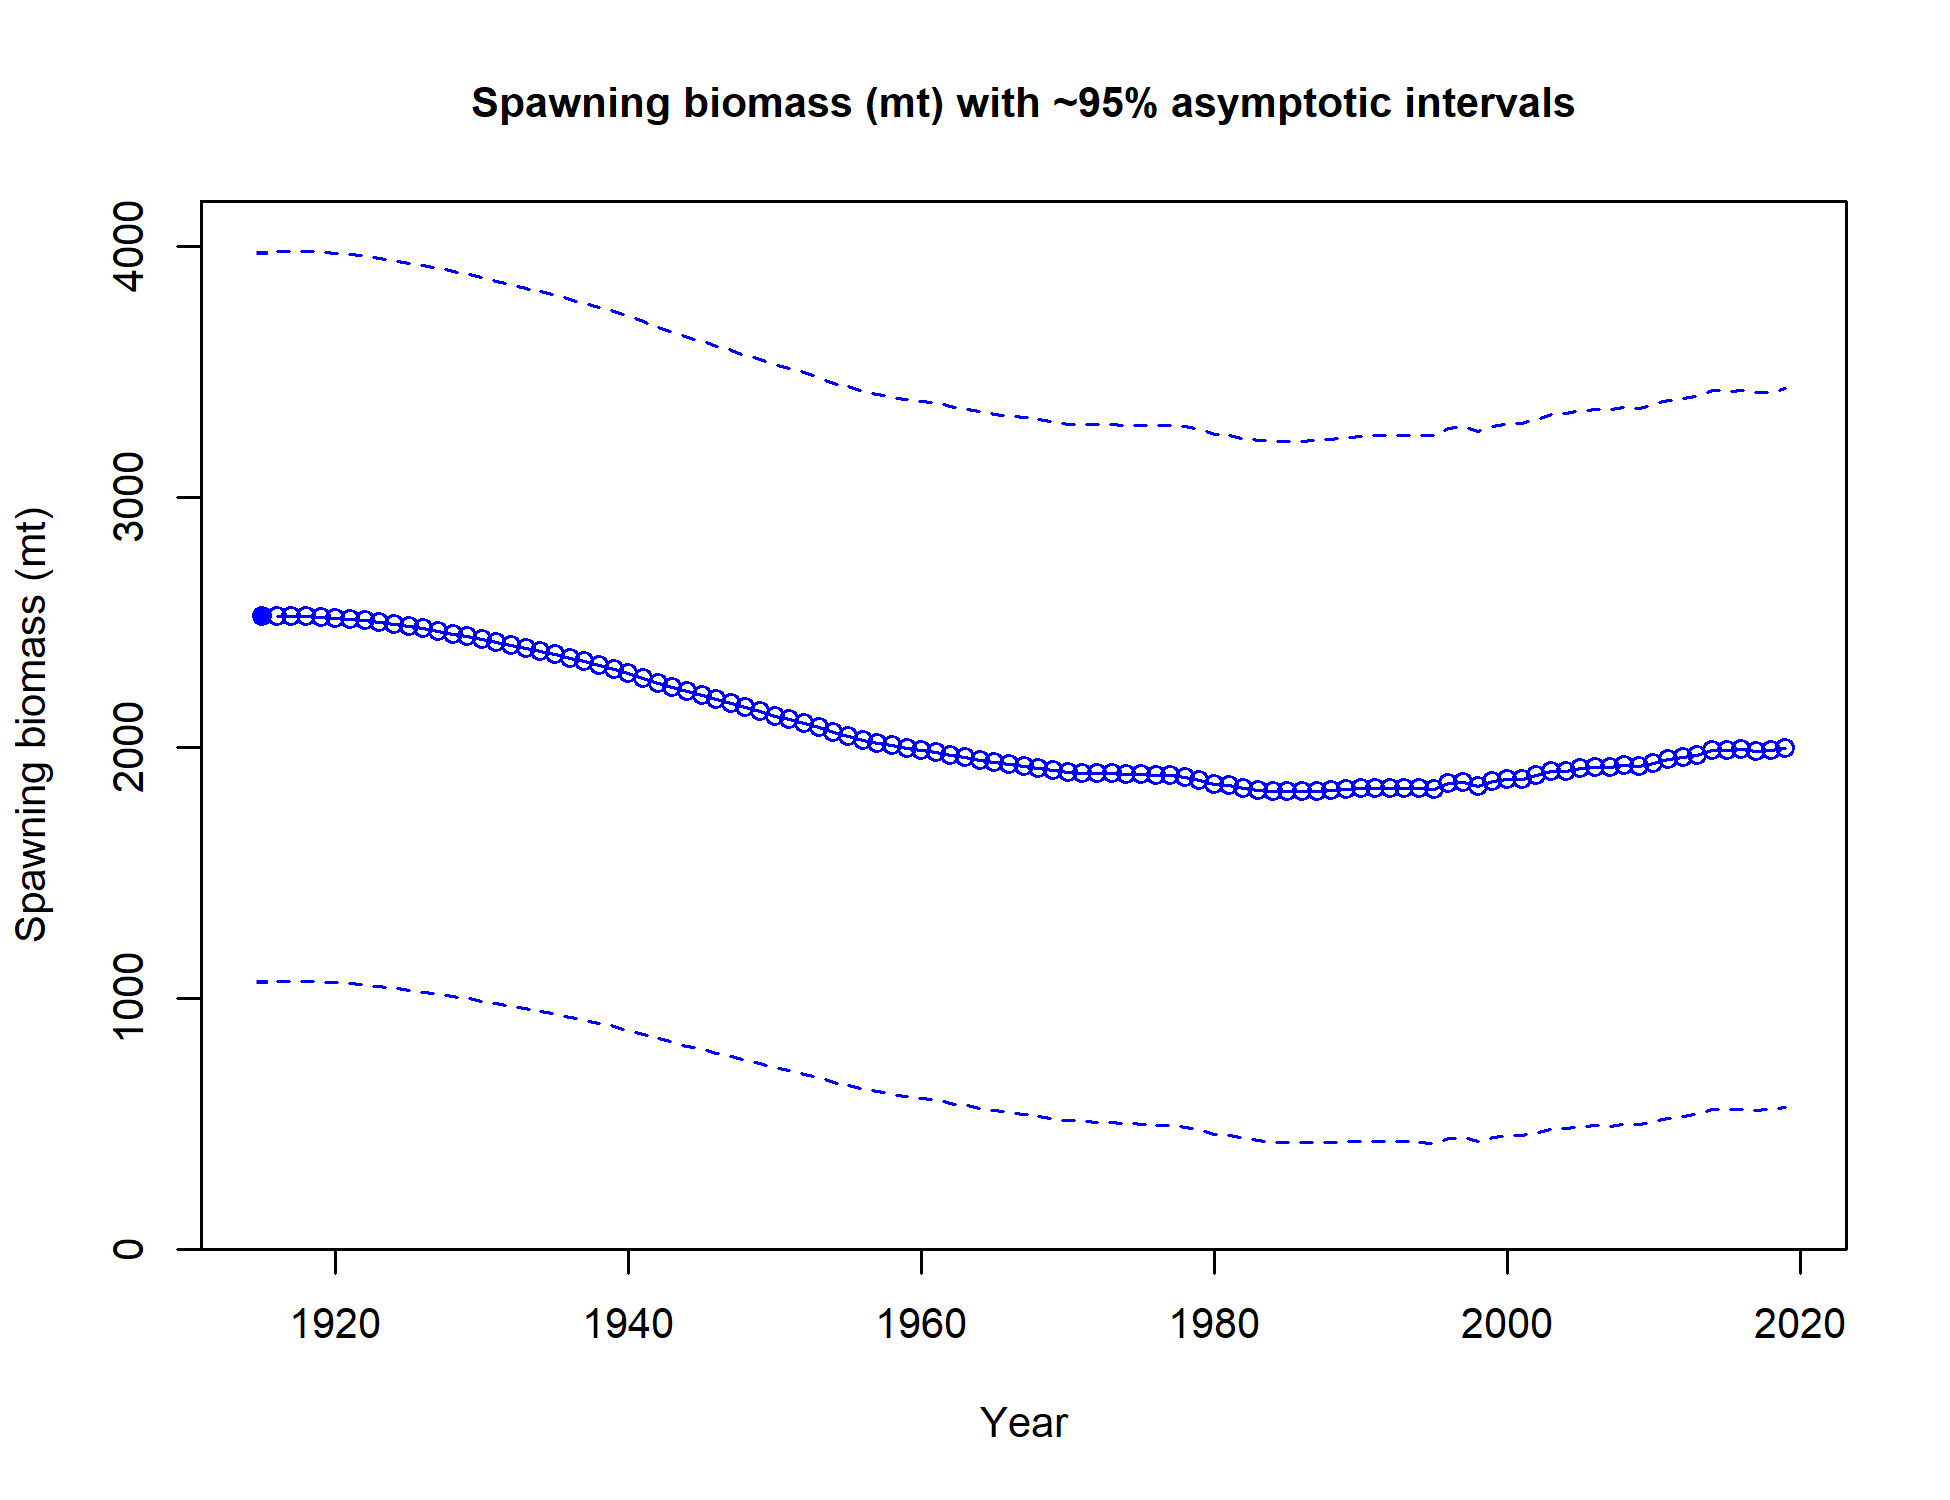
\includegraphics{r4ss/plots_mod1/ts7_Spawning_biomass_(mt)_with_95_asymptotic_intervals_intervals.png}
\caption{Time series of spawning biomass trajectory (circles and line:
median; light broken lines: 95\% credibility intervals) for the base
case assessment model. \label{fig:Spawnbio_all}}
\end{figure}

\FloatBarrier

\hypertarget{recruitment}{%
\subsection*{Recruitment}\label{recruitment}}
\addcontentsline{toc}{subsection}{Recruitment}

Recruitment was assumed to follow the Beverton-Holt stock recruit curve
with the steepness parameter fixed at \(h=0.4\), so uncertainty in
estimated recruitment is due to uncertainty in the estimated unfished
equilibrium recruitment \(R_0\) as well as uncertainty in growth and
mortality (Figure \ref{fig:Recruits_all} and Table
\ref{tab:Recruit_mod1}).

\vspace{.5cm}

\begin{table}[ht]
\centering
\caption{Recent recruitment for the model.} 
\label{tab:Recruit_mod1}
\begin{tabular}{>{\centering}p{.8in}>{\centering}p{1.6in}>{\centering}p{2in}}
  \hline
Year & Estimated Recruitment (1,000s) & \~{} 95\% confidence interval \\ 
  \hline
2010 & 6617 & (3044 - 14385) \\ 
  2011 & 6637 & (3059 - 14402) \\ 
  2012 & 6649 & (3068 - 14411) \\ 
  2013 & 6662 & (3077 - 14420) \\ 
  2014 & 6694 & (3102 - 14448) \\ 
  2015 & 6693 & (3102 - 14443) \\ 
  2016 & 6697 & (3105 - 14442) \\ 
  2017 & 6685 & (3098 - 14426) \\ 
  2018 & 6689 & (3102 - 14426) \\ 
  2019 & 6706 & (3115 - 14438) \\ 
   \hline
\end{tabular}
\end{table}

\FloatBarrier

\begin{figure}
\centering
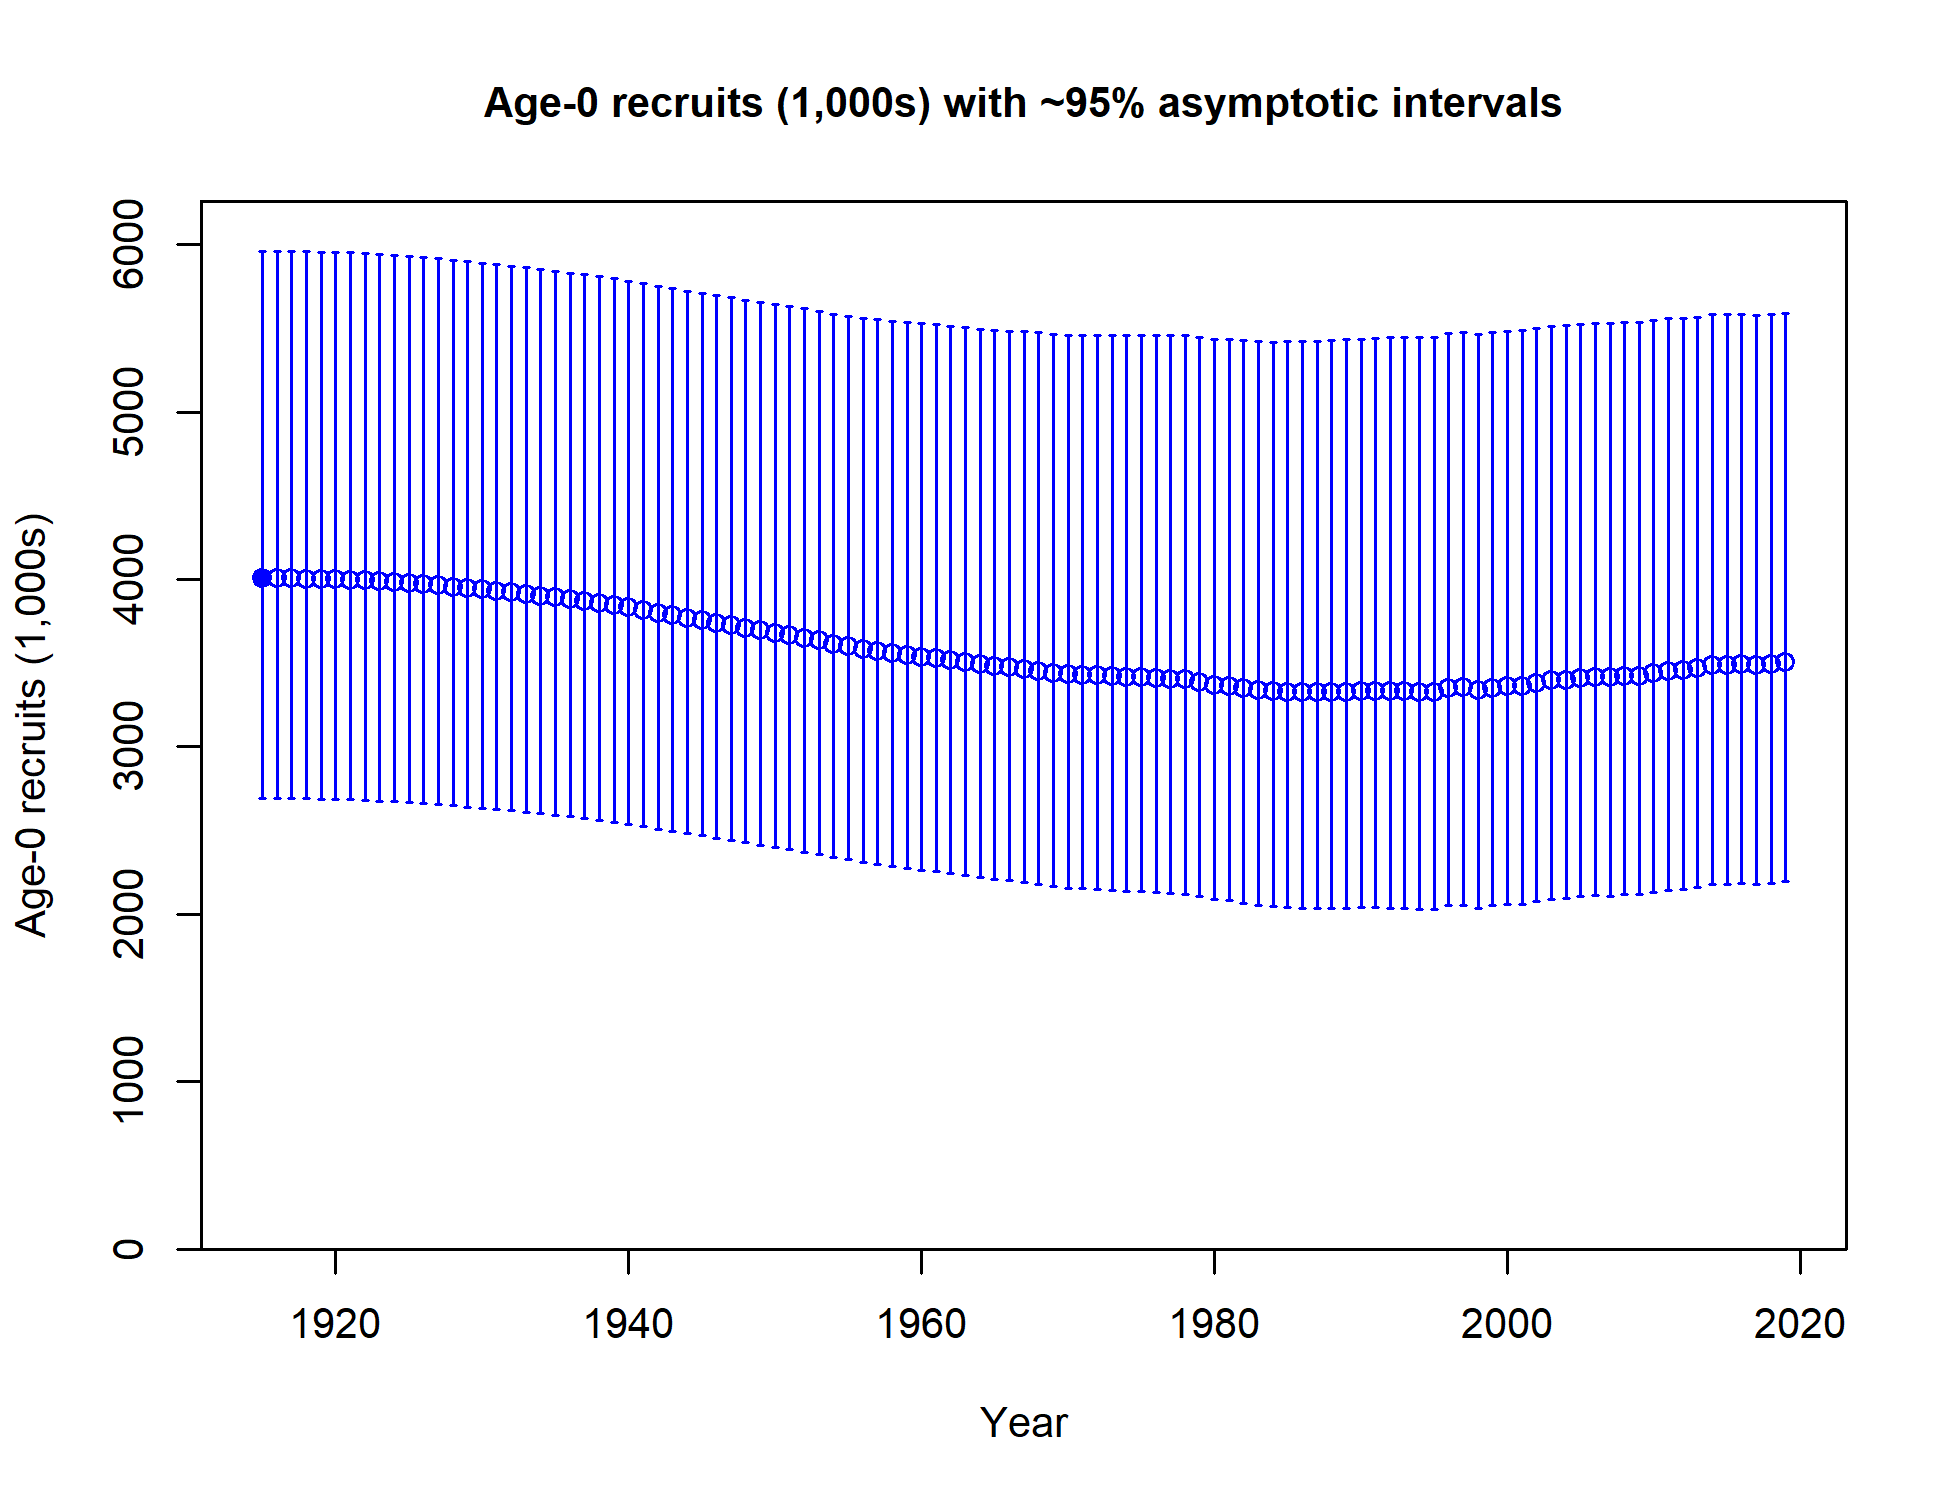
\includegraphics{r4ss/plots_mod1/ts11_Age-0_recruits_(1000s)_with_95_asymptotic_intervals.png}
\caption{Time series of estimated Big Skate recruitments for the
base-case model with 95\% confidence or credibility intervals.
\label{fig:Recruits_all}}
\end{figure}

\FloatBarrier

\hypertarget{exploitation-status}{%
\subsection*{Exploitation Status}\label{exploitation-status}}
\addcontentsline{toc}{subsection}{Exploitation Status}

Harvest rates estimated by the base model indicate catch levels have
been below the limits that would be associated with the Spawning
Potential Ratio (SPR) = 50\% limit (corresponding to a relative fishing
intensity of 100\%) (Table \ref{tab:SPR_Exploit_mod1} and Figures
\ref{fig:SPR_all} and \ref{fig:phase}). SPR is calculated as the
lifetime spawning potential per recruit at a given fishing level
relative to the lifetime spawning potential per recruit with no fishing.
The exploitation rate of age 2+ fish has been below 3\% over the recent
10-year period.

\vspace{.5cm}

\FloatBarrier

\begin{table}[ht]
\centering
\caption{Recent trend in spawning potential 
                                        ratio and exploitation for Big Skate in the model.  Relative fishing intensity is (1-SPR) 
                                        divided by 50\% (the SPR target) and exploitation 
                                        is catch divided by age 2+ biomass.} 
\label{tab:SPR_Exploit_mod1}
\begin{tabular}{l>{\centering}p{1in}>{\centering}p{1.2in}>{\centering}p{1in}>{\centering}p{1.2in}}
  \hline
Year & Relative fishing intensity & \~{} 95\% confidence interval & Exploitation rate & \~{} 95\% confidence interval \\ 
  \hline
2009 & 0.174 & (0.059-0.289) & 0.010 & (0.003-0.016) \\ 
  2010 & 0.165 & (0.057-0.273) & 0.009 & (0.003-0.015) \\ 
  2011 & 0.220 & (0.079-0.362) & 0.012 & (0.004-0.02) \\ 
  2012 & 0.220 & (0.079-0.361) & 0.012 & (0.004-0.02) \\ 
  2013 & 0.115 & (0.04-0.191) & 0.006 & (0.002-0.01) \\ 
  2014 & 0.300 & (0.114-0.486) & 0.017 & (0.006-0.028) \\ 
  2015 & 0.269 & (0.1-0.437) & 0.015 & (0.005-0.025) \\ 
  2016 & 0.332 & (0.128-0.537) & 0.019 & (0.007-0.031) \\ 
  2017 & 0.231 & (0.084-0.379) & 0.013 & (0.004-0.021) \\ 
  2018 & 0.147 & (0.052-0.243) & 0.008 & (0.003-0.013) \\ 
   \hline
\end{tabular}
\end{table}

\FloatBarrier

\begin{figure}
\centering
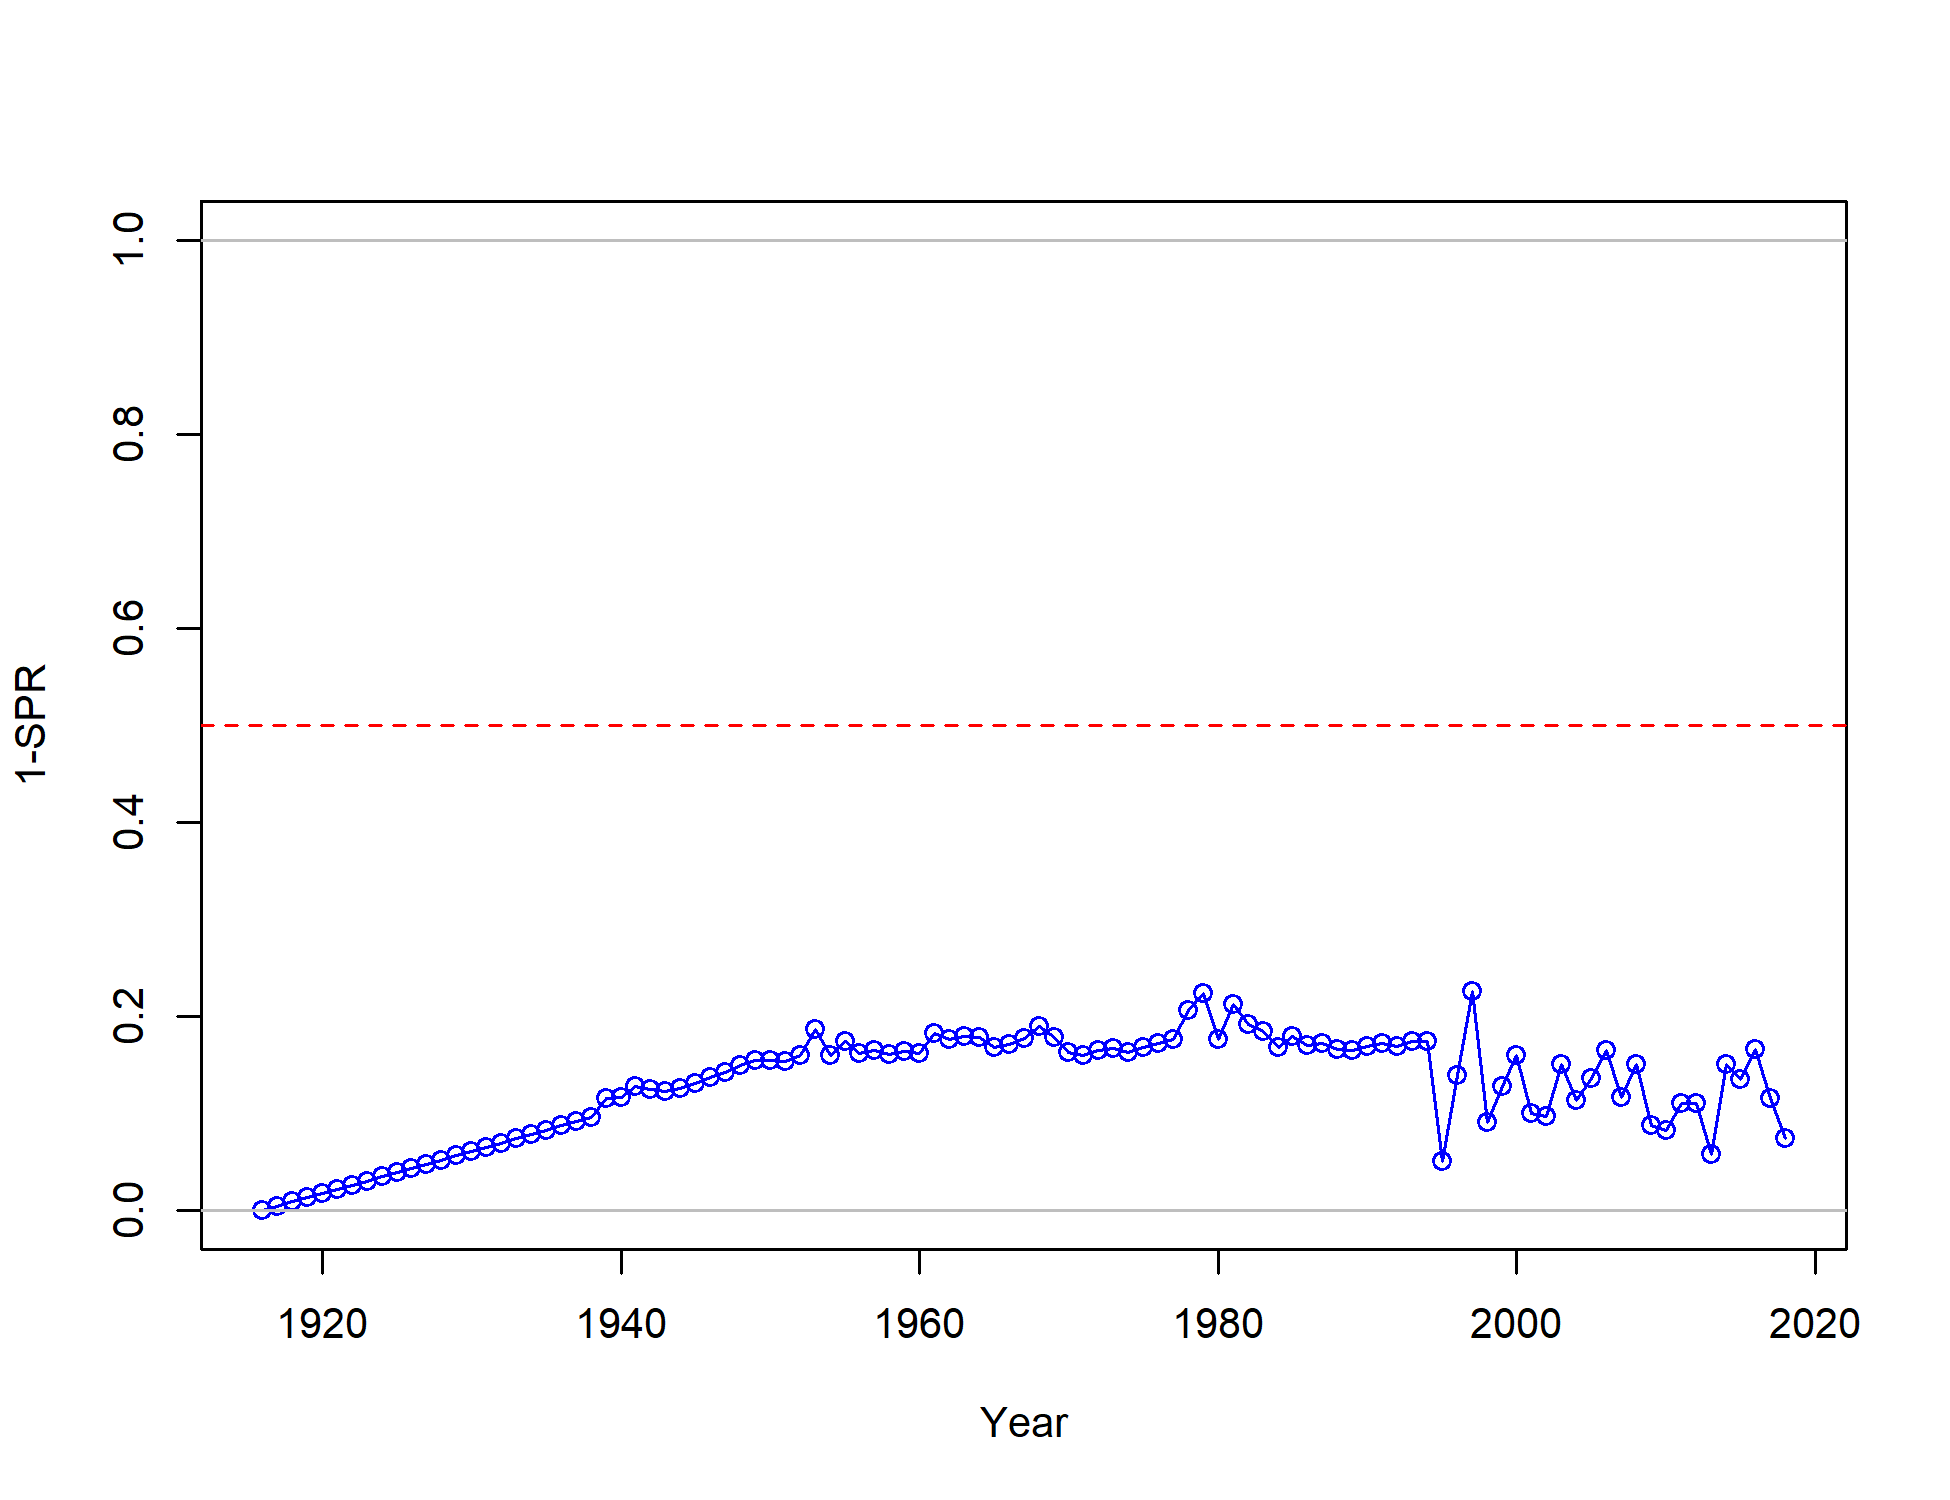
\includegraphics{r4ss/plots_mod1/SPR2_minusSPRseries.png}
\caption{Estimated Spawning Potential Ratio (SPR) for the base-case
model. One minus SPR is plotted so that higher exploitation rates occur
on the upper portion of the y-axis. The management target is plotted as
a red horizontal line and values above this reflect harvests in excess
of the overfishing proxy based on the SPR\textsubscript{50\%} harvest
rate. The last year in the time series is 2018. \label{fig:SPR_all}}
\end{figure}

\begin{figure}
\centering
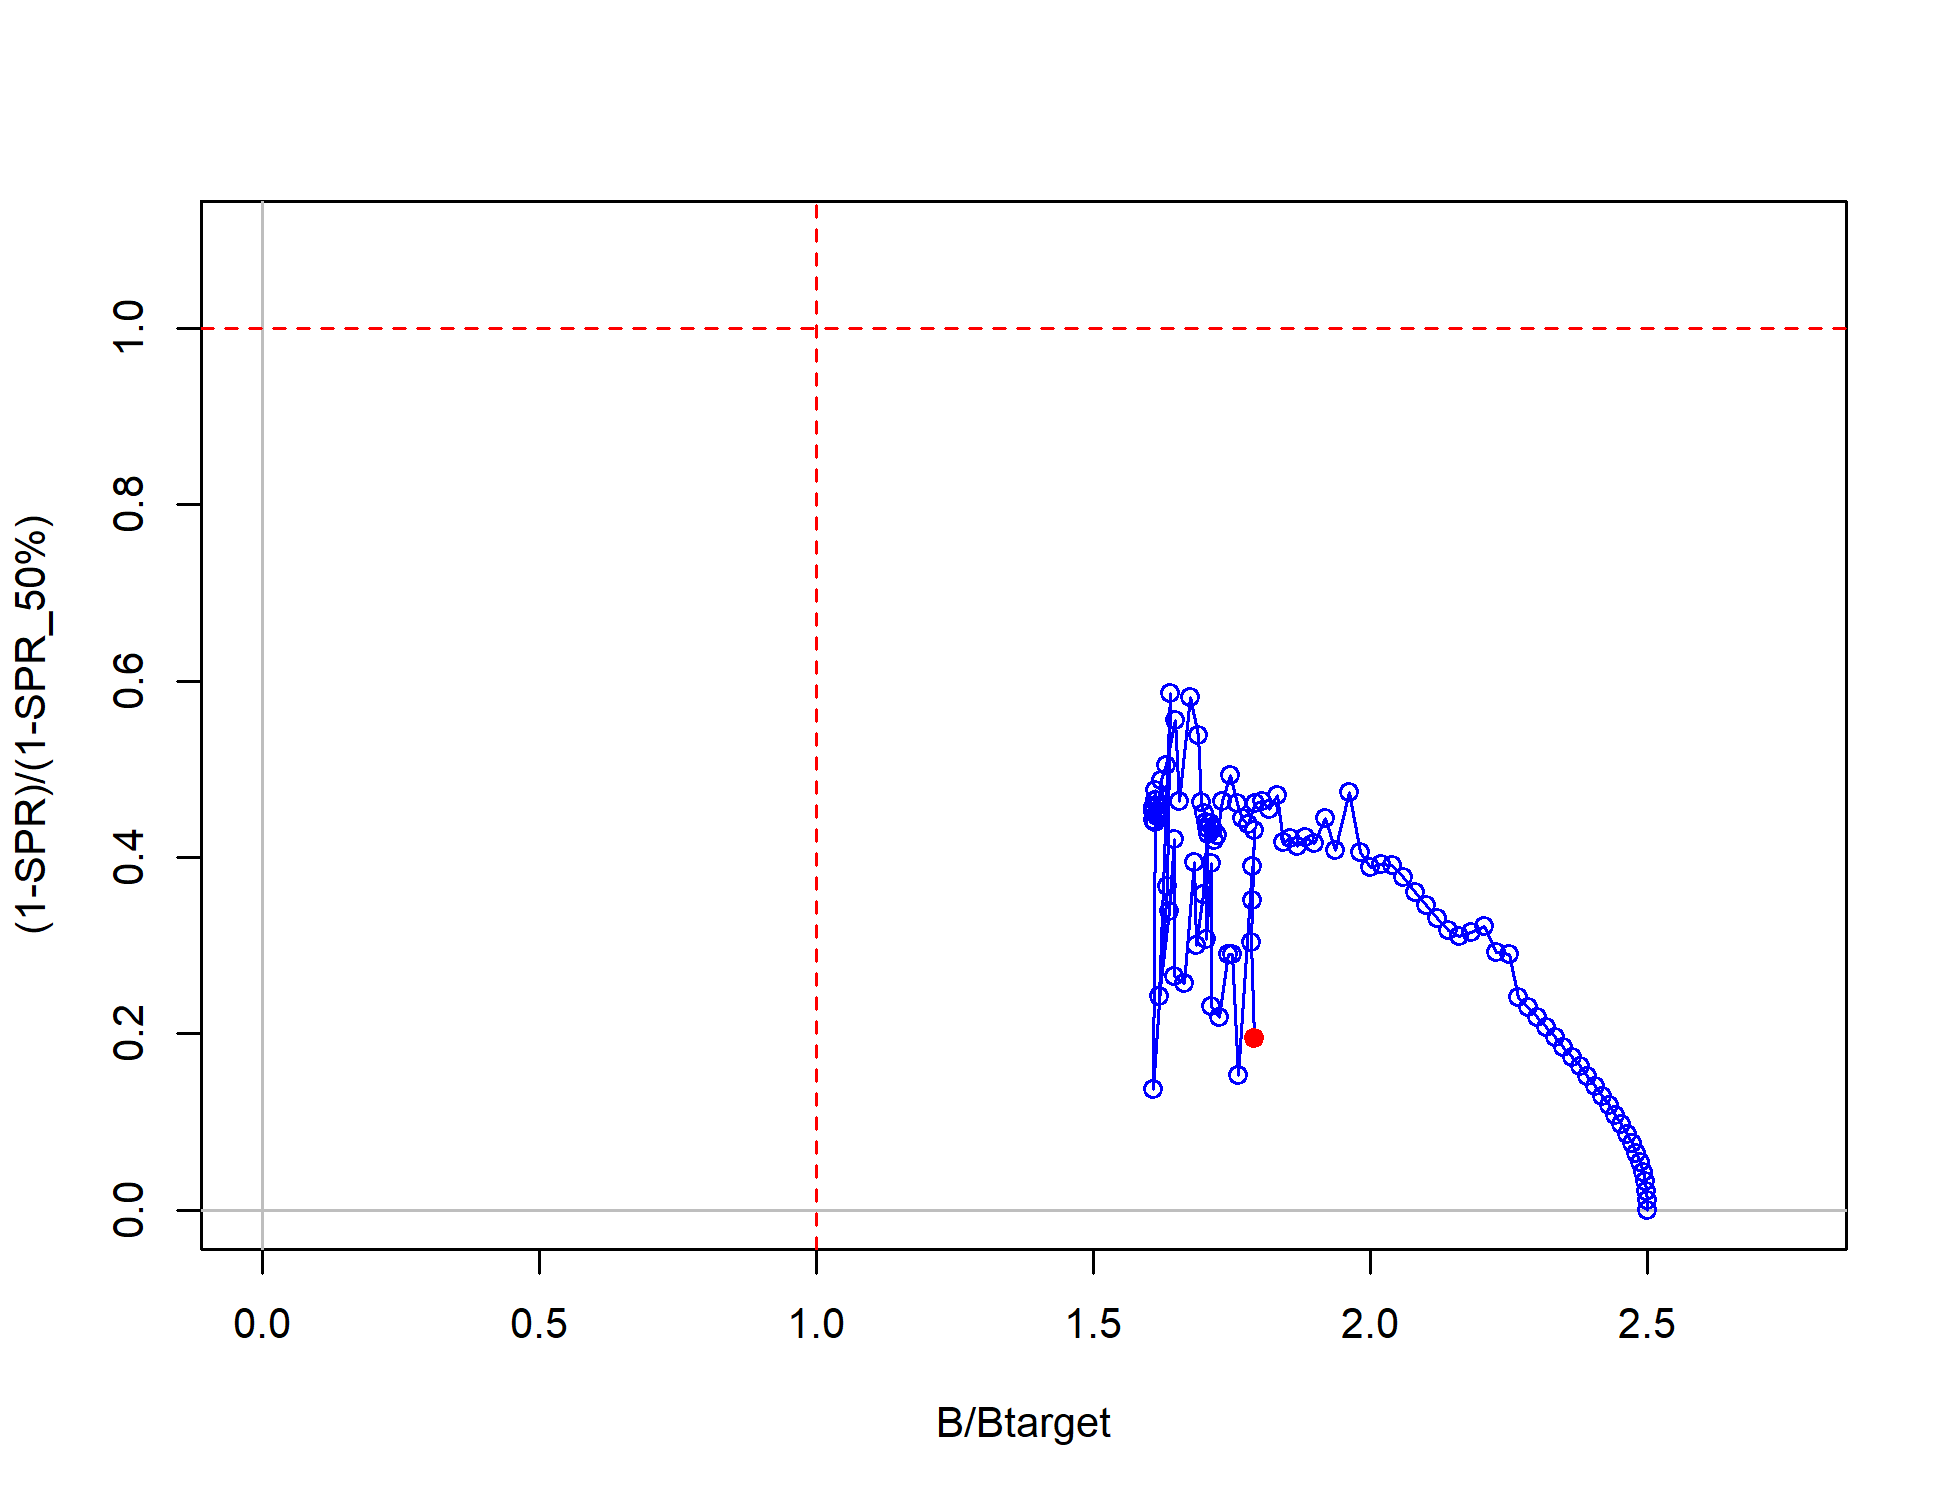
\includegraphics{r4ss/plots_mod1/SPR4_phase.png}
\caption{Phase plot of biomass vs.~fishing intensity. \label{fig:phase}}
\end{figure}

\FloatBarrier

\hypertarget{reference-points}\)), and well above the minimum stock size
threshold (\(B_{25\%}\)). The estimated \%unfished level for the base
model in 2019 is 79.2\% (95\% asymptotic interval: \(\pm\)
65.5\%-92.9\%, corresponding to an unfished spawning biomass of 1999 mt
(95\% asymptotic interval: 566-3433 mt) of spawning biomass in the base
model (Table \ref{tab:Ref_pts_mod1}). Unfished age 2+ biomass was
estimated to be 2,936 mt in the base case model. The target spawning
biomass (\(B_{40\%}\)) is 1,010 mt, which corresponds with an
equilibrium yield of 701 mt. Equilibrium yield at the proxy \(F_{MSY}\)
harvest rate corresponding to \(SPR=50\%\) is 590 mt (Figure
\ref{fig:Yield_all}).

\vspace{.5cm}

\FloatBarrier

\begin{table}[ht]
\centering
\caption{Summary of reference 
                                      points and management quantities for the 
                                      base case model.} 
\label{tab:Ref_pts_mod1}
\begin{tabular}{>{\raggedright}p{4.1in}>{\raggedleft}p{.62in}>{\raggedleft}p{.62in}>{\raggedleft}p{.62in}}
  \hline
\textbf{Quantity} & \textbf{Estimate} & \textbf{Low 2.5\%  limit} & \textbf{High 2.5\%  limit} \\ 
  \hline
Unfished spawning output (mt) & 2,525 & 1,068 & 3,981 \\ 
  Unfished age 2+ biomass (mt) & 2,936 & 1,363 & 4,509 \\ 
  Unfished recruitment ($R_{0}$, thousands) & 7,366 & 1,974 & 1,276 \\ 
  Spawning output (2018 mt) & 1,988 & 555 & 3,420 \\ 
  Depletion (2018) & 0.787 & 0.648 & 0.927 \\ 
  \textbf{$\text{Reference points based on } \mathbf{B_{40\%}}$} &  &  &  \\ 
  Spawning biomass ($B_{40\%}$) & 1,010 & 427 & 1,592 \\ 
  SPR resulting in $B_{40\%}$ ($SPR_{B40\%}$) & 0.625 & 0.625 & 0.625 \\ 
  Exploitation rate resulting in $B_{40\%}$ & 0.048 & 0.042 & 0.055 \\ 
  Yield with $SPR_{B40\%}$ at $B_{40\%}$ (mt) & 701 & 316 & 1,086 \\ 
  \textbf{\textit{Reference points based on $SPR=50\%$ proxy for MSY}} &  &  &  \\ 
  Spawning biomass (mt) & 505 & 214 & 796 \\ 
  $SPR_{proxy}$ & 0.5 &  &  \\ 
  Exploitation rate corresponding to $SPR=50\%$ & 0.071 & 0.061 & 0.08 \\ 
  Yield with $SPR=50\%$ at $B_{SPR=50\%}$ (mt) & 590 & 266 & 915 \\ 
  \textbf{\textit{Reference points based on estimated MSY values}} &  &  &  \\ 
  Spawning biomass at $MSY$ ($B_{MSY}$) & 944 & 393 & 1,496 \\ 
  $SPR_{MSY}$ & 0.609 & 0.604 & 0.614 \\ 
  Exploitation rate at $MSY$ & 0.051 & 0.045 & 0.057 \\ 
  Dead Catch $MSY$ (mt) & 703 & 316 & 1,089 \\ 
  Retained Catch $MSY$ (mt) & 650 & 294 & 1,005 \\ 
   \hline
\end{tabular}
\end{table}

\FloatBarrier

\newpage

\hypertarget{ecosystem-considerations}{%
\subsection*{Ecosystem Considerations}\label{ecosystem-considerations}}
\addcontentsline{toc}{subsection}{Ecosystem Considerations}

Big Skate have broad thermal tolerances and are broadly distributed,
occurring from the southeastern Bering Sea to southern Baja California
and the Gulf of California. They have been reported at depths of 2-501 m
but are most common on the inner continental shelf (\textless{} 100 m).
Big Skates are opportunistic predators with highly variable
spatio-temporal trophic roles.

In this assessment, neither environmental nor ecosystem considerations
were explicitly included in the analysis. This is primarily due to a
lack of relevant data or results of analyses that could contribute
ecosystem-related quantitative information for the assessment.

\hypertarget{management-performance}{%
\subsection*{Management Performance}\label{management-performance}}
\addcontentsline{toc}{subsection}{Management Performance}

Annual Catch Limits have only been in place for Big Skate in recent
years and total catch, including discards has remained below these
limits with the exception of 2014, where in retrospect the catch was
above the ACL although still below the Overfishing Limit (Table
\ref{tab:mnmgt_perform}).

\begin{table}[ht]
\centering
\caption{Recent trend in total catch (mt) relative to the 
                              management guidelines. Big skate was
                              managed in the Other Species complex in 2013 and 2014,
                              designated an Ecosystem Component species in 2015 and
                              2016, and managed with stock-specific harvest
                              specifications since 2017. Estimated total mortality
                              includes discards estimated in the model with an
                              assumed mortality rate of 50\%.} 
\label{tab:mnmgt_perform}
\scalebox{0.9}{
\begin{tabular}{l>{\centering}p{1.2in}>{\centering}p{1in}>{\centering}p{1in}>{\centering}p{1in}>{\centering}p{1in}}
  \hline
Year & OFL (mt; ABC prior to 2011) & ABC (mt) & ACL (mt; OY prior to 2011) & Landings (mt) & Estimated total mortality (mt) \\ 
  \hline
2009 &  &  &  & 205.7 & 217.2 \\ 
  2010 &  &  &  & 196.2 & 206.6 \\ 
  2011 &  &  &  & 268.4 & 282.0 \\ 
  2012 &  &  &  & 269.6 & 282.4 \\ 
  2013 & 458 & 317.9 & 317.9 & 135.0 & 144.3 \\ 
  2014 & 458 & 317.9 & 317.9 & 372.5 & 396.9 \\ 
  2015 &  &  &  & 331.6 & 350.6 \\ 
  2016 &  &  &  & 411.5 & 440.7 \\ 
  2017 & 541 & 494.0 & 494.0 & 277.6 & 297.2 \\ 
  2018 & 541 & 494.0 & 494.0 & 172.6 & 185.4 \\ 
  2019 & 541 & 494.0 & 494.0 &  &  \\ 
  2020 & 541 & 494.0 & 494.0 &  &  \\ 
   \hline
\end{tabular}
}
\end{table}

\FloatBarrier

\hypertarget{unresolved-problems-and-major-uncertainties}{%
\subsection*{Unresolved Problems and Major
Uncertainties}\label{unresolved-problems-and-major-uncertainties}}
\addcontentsline{toc}{subsection}{Unresolved Problems and Major
Uncertainties}

The data provide little information about the scale of the population,
necessitating the use of a prior on catchability to maintain stable
model results. The prior was developed for the 2007 Longnose Skate stock
assessment and has not been revised to account for any differences
between the two species.

There is little evidence that the population is overfished or
experiencing overfishing, but forecasts of overfishing limits vary
considerably among the sensitivity analyses explored (though all remain
well above the recent average catch).

The fit to the length data was significantly improved by estimating a
difference between female and male selectivity, with females having a
lower maximum selectivity than males, but the behavioral processes that
might contribute to this difference are not understood.

\FloatBarrier

\hypertarget{decision-table}{%
\subsection*{Decision Table}\label{decision-table}}
\addcontentsline{toc}{subsection}{Decision Table}

\textbf{\(\color{red}{\text{Template in Table h and associated discussion to be filled in during the STAR panel}}\)}

\FloatBarrier

\hypertarget{projected-landings-ofls-and-time-varying-acls}{%
\subsection*{Projected Landings, OFLs and Time-varying
ACLs}\label{projected-landings-ofls-and-time-varying-acls}}
\addcontentsline{toc}{subsection}{Projected Landings, OFLs and
Time-varying ACLs}

Potential OFLs projected by the model are shown in Table
\ref{tab:OFL_projection_Exec}. These values are based on an SPR target
of 50\%, a P* of 0.45, and a time-varying Category 2 Sigma which creates
the buffer shown in the right-hand column. The OFL and ACL values for
2019 and 2020 are the current harvest specifications (also shown in
Table \ref{tab:mnmgt_perform}) while the landings for 2019 and 2020
represent the average landings over the most recent 5 years
(2014--2018).

\begin{table}[ht]
\centering
\caption{Projections of landings, total mortality, OFL, and ACL values.} 
\label{tab:OFL_projection_Exec}
\begin{tabular}{l>{\centering}p{0.8in}>{\centering}p{1.2in}>{\centering}p{0.8in}>{\centering}p{0.8in}>{\centering}p{0.8in}}
  \hline
Year & Landings (mt) & Estimated total mortality (mt) & OFL (mt) & ACL (mt) & Buffer \\ 
  \hline
2019 & 313.2 & 336.3 & 541.0 & 494.0 & 1.000 \\ 
  2020 & 313.2 & 336.3 & 541.0 & 494.0 & 1.000 \\ 
  2021 & 1370.7 & 1472.8 & 1677.0 & 1472.8 & 0.874 \\ 
  2022 & 1288.6 & 1387.2 & 1595.6 & 1387.2 & 0.865 \\ 
  2023 & 1224.5 & 1320.4 & 1532.5 & 1320.4 & 0.857 \\ 
  2024 & 1174.9 & 1268.1 & 1485.2 & 1268.1 & 0.849 \\ 
  2025 & 1135.7 & 1226.0 & 1449.2 & 1226.0 & 0.841 \\ 
  2026 & 1101.9 & 1189.5 & 1419.0 & 1189.5 & 0.833 \\ 
  2027 & 1071.9 & 1156.8 & 1391.4 & 1156.8 & 0.826 \\ 
  2028 & 1041.5 & 1123.8 & 1364.5 & 1123.8 & 0.818 \\ 
  2029 & 1011.7 & 1091.5 & 1338.0 & 1091.5 & 0.810 \\ 
  2030 & 983.7 & 1061.1 & 1311.7 & 1061.1 & 0.803 \\ 
   \hline
\end{tabular}
\end{table}
\begin{table}[ht]
\centering
\caption{Summary of 10-year 
                                             projections beginning in 2020 
                                             for alternate states of nature based on 
                                             an axis of uncertainty for the model.  Columns range over low, mid, and high
                                             states of nature, and rows range over different 
                                             assumptions of catch levels. An entry of "--" 
                                             indicates that the stock is driven to very low 
                                             abundance under the particular scenario.} 
\label{tab:Decision_table_mod1}
\scalebox{0.85}{
\begin{tabular}{l|cc|>{\centering}p{.7in}c|>{\centering}p{.7in}c|>{\centering}p{.7in}c}
   \multicolumn{3}{c}{}  &  \multicolumn{2}{c}{} 
                               & \multicolumn{2}{c}{\textbf{States of nature}} 
                               & \multicolumn{2}{c}{} \\
  \multicolumn{3}{c}{}  &  \multicolumn{2}{c}{Low State} 
                               & \multicolumn{2}{c}{Base State} 
                               &  \multicolumn{2}{c}{High State} \\
 \hline
 & Year & Catch & Spawning Output & Depletion & Spawning Output & Depletion & Spawning Output & Depletion \\ 
  \hline
 & 2019 & - & - & - & - & - & - & - \\ 
   & 2020 & - & - & - & - & - & - & - \\ 
   & 2021 & - & - & - & - & - & - & - \\ 
  Default harvest,  & 2022 & - & - & - & - & - & - & - \\ 
  for Low State & 2023 & - & - & - & - & - & - & - \\ 
   & 2024 & - & - & - & - & - & - & - \\ 
   & 2025 & - & - & - & - & - & - & - \\ 
   & 2026 & - & - & - & - & - & - & - \\ 
   & 2027 & - & - & - & - & - & - & - \\ 
   & 2028 & - & - & - & - & - & - & - \\ 
   \hline
 & 2019 & - & - & - & - & - & - & - \\ 
   & 2020 & - & - & - & - & - & - & - \\ 
   & 2021 & - & - & - & - & - & - & - \\ 
  Default harvest,  & 2022 & - & - & - & - & - & - & - \\ 
  for Base State & 2023 & - & - & - & - & - & - & - \\ 
   & 2024 & - & - & - & - & - & - & - \\ 
   & 2025 & - & - & - & - & - & - & - \\ 
   & 2026 & - & - & - & - & - & - & - \\ 
   & 2027 & - & - & - & - & - & - & - \\ 
   & 2028 & - & - & - & - & - & - & - \\ 
   \hline
 & 2019 & - & - & - & - & - & - & - \\ 
   & 2020 & - & - & - & - & - & - & - \\ 
   & 2021 & - & - & - & - & - & - & - \\ 
  Default harvest,  & 2022 & - & - & - & - & - & - & - \\ 
  for High State & 2023 & - & - & - & - & - & - & - \\ 
   & 2024 & - & - & - & - & - & - & - \\ 
   & 2025 & - & - & - & - & - & - & - \\ 
   & 2026 & - & - & - & - & - & - & - \\ 
   & 2027 & - & - & - & - & - & - & - \\ 
   & 2028 & - & - & - & - & - & - & - \\ 
   \hline
 & 2019 & - & - & - & - & - & - & - \\ 
   & 2020 & - & - & - & - & - & - & - \\ 
   & 2021 & - & - & - & - & - & - & - \\ 
  Average & 2022 & - & - & - & - & - & - & - \\ 
  Catch & 2023 & - & - & - & - & - & - & - \\ 
   & 2024 & - & - & - & - & - & - & - \\ 
   & 2025 & - & - & - & - & - & - & - \\ 
   & 2026 & - & - & - & - & - & - & - \\ 
   & 2027 & - & - & - & - & - & - & - \\ 
   & 2028 & - & - & - & - & - & - & - \\ 
   \hline
\end{tabular}
}
\end{table}
\FloatBarrier

\newgeometry{hmargin=1in,vmargin=1in}

\begin{landscape}

\renewcommand{\arraystretch}{1.2}
\begin{table}[ht]
\centering
\caption{Base case results summary.} 
\label{tab:base_summary}
\scalebox{0.6}{
\begin{tabular}{r>{\centering}p{1.1in}>{\centering}p{1.1in}>{\centering}p{1.1in}>{\centering}p{1.1in}>{\centering}p{1.1in}>{\centering}p{1.1in}>{\centering}p{1.1in}>{\centering}p{1.1in}>{\centering}p{1.1in}>{\centering}p{1.1in}}
  \hline
Quantity & 2010 & 2011 & 2012 & 2013 & 2014 & 2015 & 2016 & 2017 & 2018 & 2019 \\ 
  \hline
Landings (mt) &  313.2 &  313.2 & 1370.7 & 1288.6 & 1224.5 & 1174.9 & 1135.7 & 1101.9 & 1071.9 & 1041.5 \\ 
  Total Est. Catch (mt) &  336.3 &  336.3 & 1472.8 & 1387.2 & 1320.4 & 1268.1 & 1226.0 & 1189.5 & 1156.8 & 1123.8 \\ 
  OFL (mt) &  541.0 &  541.0 & 1677.0 & 1595.6 & 1532.5 & 1485.2 & 1449.2 & 1419.0 & 1391.4 & 1364.5 \\ 
  ACL (mt) &  494.0 &  494.0 & 1472.8 & 1387.2 & 1320.4 & 1268.1 & 1226.0 & 1189.5 & 1156.8 & 1123.8 \\ 
   \hline
(1-$SPR$)(1-$SPR_{50\%}$) & 0.16 & 0.22 & 0.22 & 0.12 & 0.30 & 0.27 & 0.33 & 0.23 & 0.15 &  \\ 
   \hline
Exploitation rate & 0.01 & 0.01 & 0.01 & 0.01 & 0.02 & 0.02 & 0.02 & 0.01 & 0.01 &  \\ 
  Age 2+ biomass (mt) & 22838.5 & 22993.9 & 23136.9 & 23191.8 & 23240.0 & 23409.4 & 23327.4 & 23308.8 & 23217.2 & 23278.8 \\ 
   \hline
Spawning Output & 1938.7 & 1952.3 & 1960.1 & 1969.0 & 1991.1 & 1990.4 & 1992.8 & 1984.9 & 1987.9 & 1999.3 \\ 
  ~95\% CI & (507.5-3369.9) & (519.8-3384.9) & (527.3-3393) & (535.8-3402.1) & (556-3426.2) & (556.3-3424.5) & (559.1-3426.6) & (552.5-3417.3) & (555.4-3420.4) & (565.7-3433) \\ 
   \hline
Depletion & 0.8 & 0.8 & 0.8 & 0.8 & 0.8 & 0.8 & 0.8 & 0.8 & 0.8 & 0.8 \\ 
  ~95\% CI & (0.616-0.92) & (0.624-0.922) & (0.628-0.924) & (0.634-0.926) & (0.648-0.93) & (0.647-0.929) & (0.649-0.929) & (0.645-0.927) & (0.647-0.927) & (0.655-0.929) \\ 
   \hline
Recruits & 6617 & 6637 & 6649 & 6662 & 6694 & 6693 & 6697 & 6685 & 6689 & 6706 \\ 
  ~95\% CI & (3044 - 14385) & (3059 - 14402) & (3068 - 14411) & (3077 - 14420) & (3102 - 14448) & (3102 - 14443) & (3105 - 14442) & (3098 - 14426) & (3102 - 14426) & (3115 - 14438) \\ 
   \hline
\end{tabular}
}
\end{table}
\renewcommand{\arraystretch}{1}
\end{landscape}
\restoregeometry

\begin{figure}
\centering
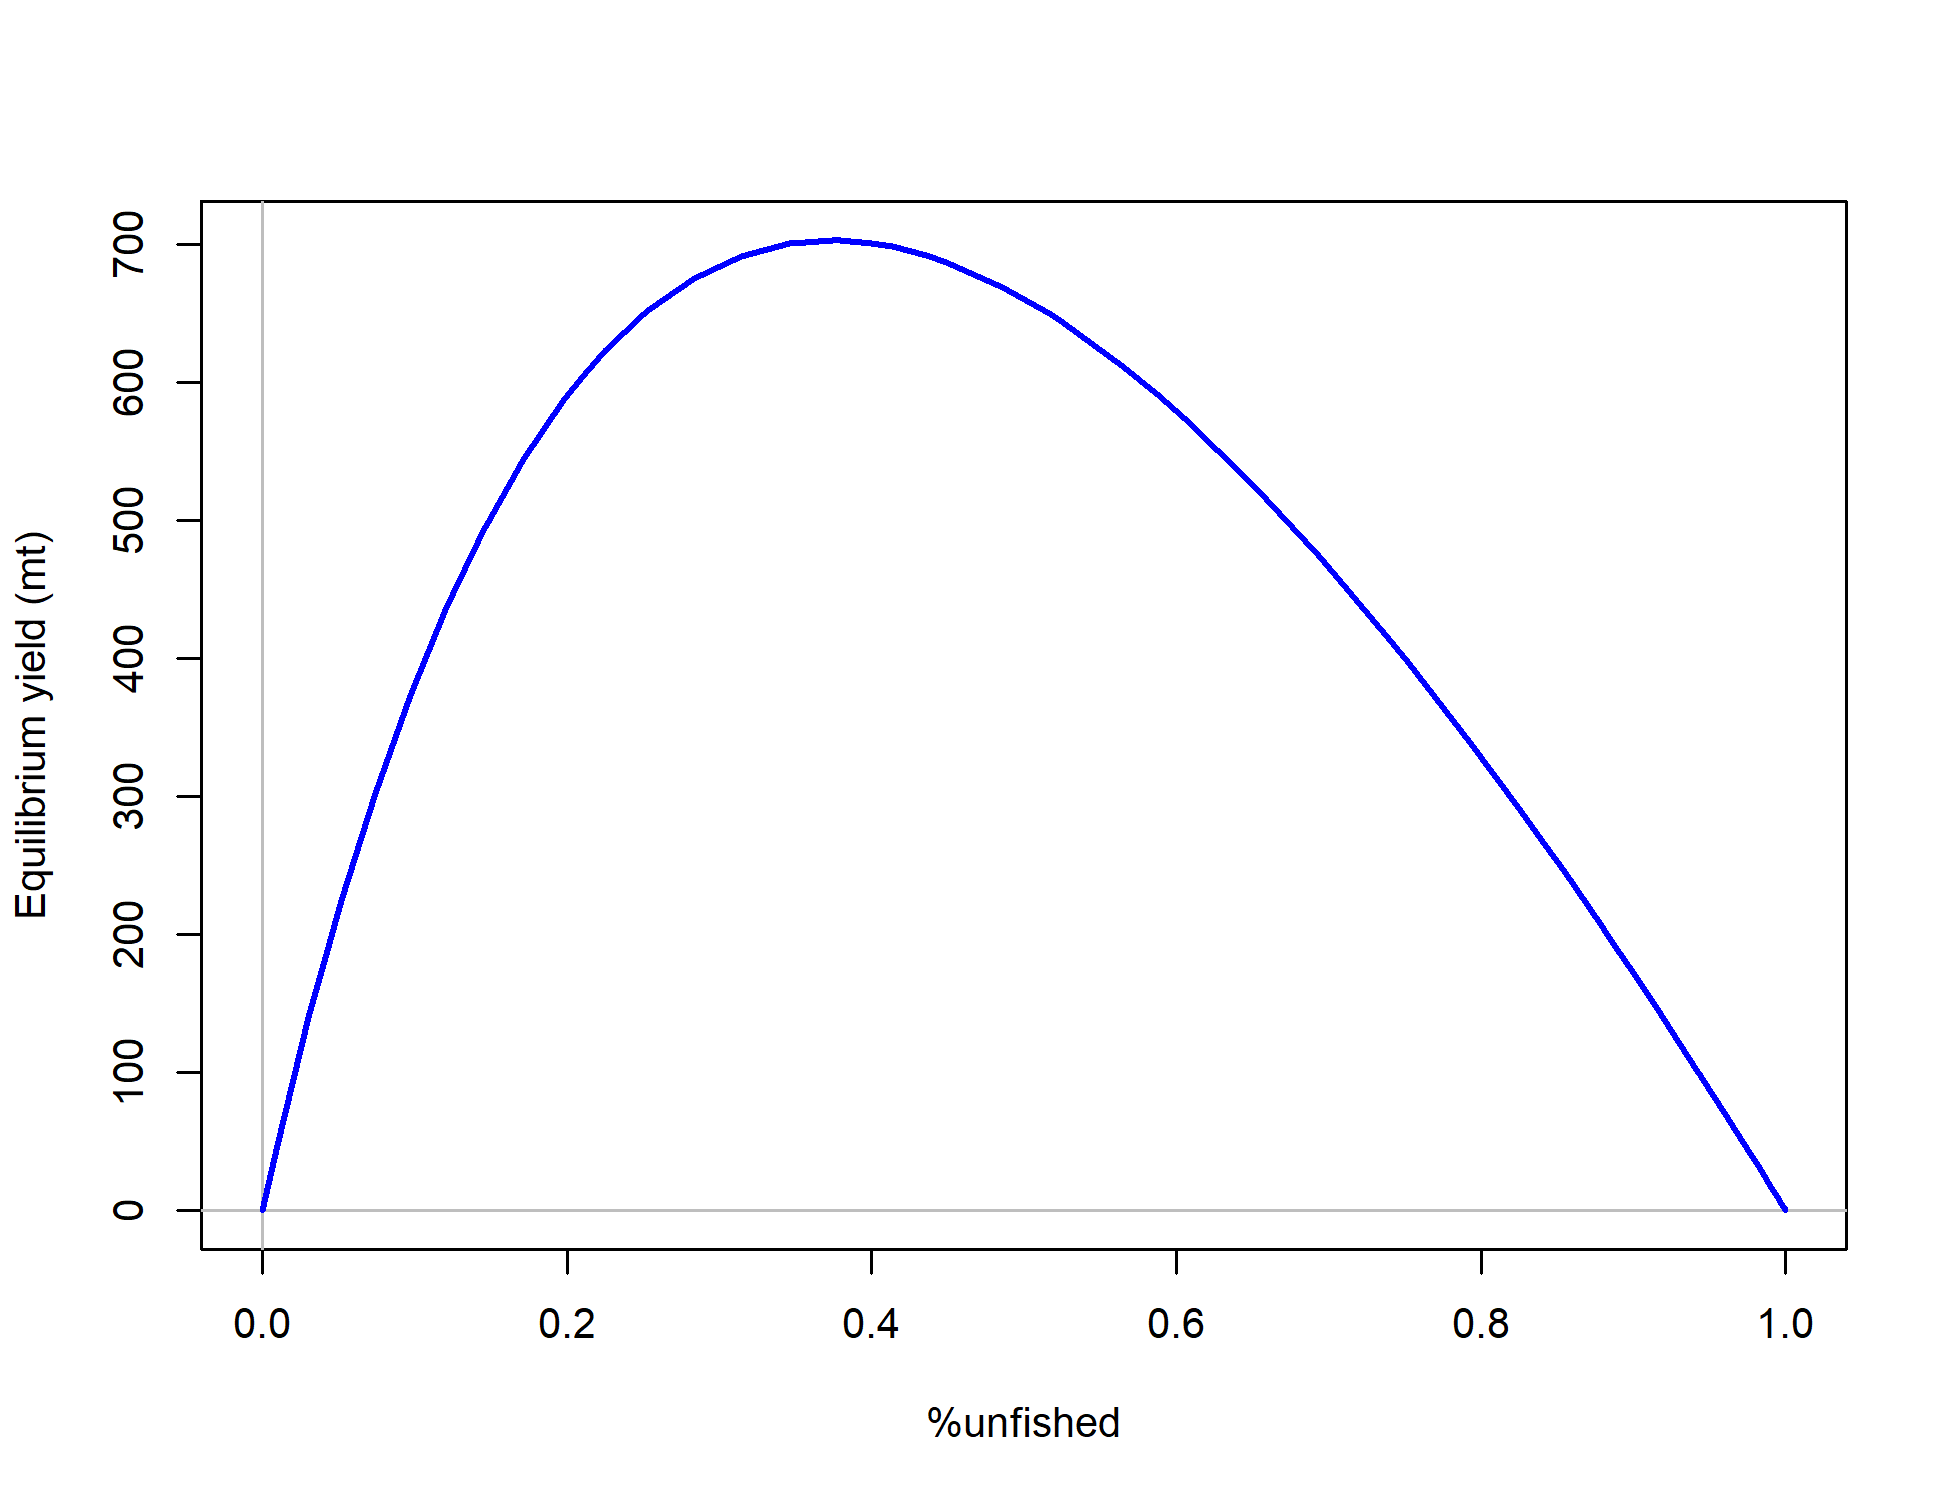
\includegraphics{r4ss/plots_mod1/yield1_yield_curve.png}
\caption{Equilibrium yield curve for the base case model. Values are
based on the 2018 fishery selectivity and retention with steepness fixed
at 0.4. \label{fig:Yield_all}}
\end{figure}

\FloatBarrier

\newpage

\hypertarget{research-and-data-needs}{%
\subsection*{Research and Data Needs}\label{research-and-data-needs}}
\addcontentsline{toc}{subsection}{Research and Data Needs}

We recommend the following research be conducted before the next
assessment.

\begin{enumerate}

\item \textbf{Extend all ongoing data streams used in this assessment.} A longer fishery-independent index from a continued WCGBT Survey with associated compositions of length and age-at-length will improve understanding of dynamics of the stock. Continued sampling of lengths and ages from the landed catch and lengths, mean body weights, and discard rates from the fishery will be even more valuable for the years ahead now that Big Skate are landed as a separate market category and the estimates will be more precise.

\item \textbf{Investigate factors contributing to estimated lower selectivity for females than males.} Sex-specific differences in selectivity were included in the base model to better fit differences in sex ratios in the length composition data but the behavioral processes that might contribute to this pattern are not understood and other explanations for the sex ratios are possible.

\item \textbf{Investigate the distribution of Big Skate shallower than the 55 m limit of the WCGBT Survey.} This would help with interpretation of the biomass estimates from the survey and potentially refining the associated prior on catchability.

\item \textbf{Pursue additional approaches for estimating historical discards.} The approaches used here were based on averages applied over a period of decades. The catch reconstructions conducted for each state were much more sophisticated, but were applied only to the subset of the catch that was landed. Reconstructed spatial patterns of fishing effort could be used to estimate changes in total mortality over time.

\item \textbf{Improve understanding of links between Big Skate on the U.S. West Coast and other areas.} Tagging studies in Alaska indicated that Big Skate are capable of long distance movements. A better understanding of links through tagging in other areas and genetic studies could highlight strengths or weaknesses of the status-quo approach.

\item \textbf{Conduct studies of mortality of discarded skates in commercial fisheries.} Estimates of discard mortality for skates in general could be improved.

\item \textbf{Improve understanding of catch history and population dynamics of California Skate.} California Skate is the third most commonly occurring Skate in California waters after Longnose Skate and Big Skate and the catch reconstruction indicated that the center of abundance for California Skate is centered around San Francisco, where the fishery was strongest in the early years. If California Skate is found to be at a low biomass compared to historical levels it would have implications for the catch reconstruction of the other two species, as well as suggesting that management of California Skate should be a higher priority.

\end{enumerate}

\FloatBarrier

\newpage
\renewcommand{\thefigure}{\arabic{figure}}
\renewcommand{\thetable}{\arabic{table}}
\setcounter{figure}{0}
\setcounter{table}{0}

\hypertarget{refs}{}
\leavevmode\hypertarget{ref-Gertseva2007}{}%
Gertseva, V and Schirippa, MJ. 2007. Status of the Longnose Skate
(\emph{Raja rhina}) off the continental US Pacific Coast in 2007.
Pacific Fishery Management Council, Portland, OR. Available from
\href{\%7Bhttp://www.pcouncil.org/groundfish/stock-assessments/\%7D}{\{http://www.pcouncil.org/groundfish/stock-assessments/\}}.

\end{document}
